\chapter{Edges}
\label{chap:power}
\begin{figure}
  \centering
  \includegraphics[width=\textwidth]{power/unity.png}
  \caption[The Unity game engine, visualised using the Unity game engine]{A visualisation of the Unity game engine, rendered using the Unity game engine. 
  Edges are bundled using hierarchical edge bundling as described in Section~\ref{sec:heb_background}. The graph has a total of 5,025 vertices and 20,177 edges, reduced to 8,380 included in the final render to reduce clutter. The colour applied to each edge highlights the class being referenced by transitioning from light to dark, in order to emphasise the pattern of certain important nodes that many others depend on. For example, the thickest bundle in the top right comes from a folder called \texttt{Math/}, which is used in calculations all over the source code. The thick bundle coming from the top left is a folder called \texttt{IMGUI/}, which is used for debugging with developer tools.
  Using \texttt{MAX\_EXT} blending as suggested by Holten \cite{Holten2006} allows links flowing in opposite directions to be salient, and anti-aliasing is crucial for smoothing the output.}
  \label{fig:metaunity}
\end{figure}
The previous chapter was an exploration of how to position the vertices of a graph, and the natural question to then ask is how to deal with the only remaining component: the edges. However this question is seemingly redundant at first, as the obvious answer is to simply draw straight lines between adjacent nodes. While this by no means a poor choice, and is exactly how all node-link diagrams have been drawn thus far, this chapter will explore the possibility of drawing links using curves instead.

\section{Background}
\label{sec:edges_background}
The curving of links in the context of a node-link diagram is known as \textit{edge bundling}. It is a technique that has been developed because many networks, when processed through a standard force-directed layout, result in a seemingly random layout with no discernable structure. See Figure~\ref{fig:untangled_hairballs} for examples of this. The similarity of such layouts to tangled collections of hair has led to them being colloquially termed \textit{hairballs}.

Unfortunately this is not an easily solved problem, because the \textit{curse of dimensionality} \cite{Friedman2001Local} means that most of these networks simply cannot be accurately represented in two dimensions, and the likelihood of this problem only rises as the size of any network increases. This can happen even if there exists a clear underlying structure to these networks, lying beyond the reach of the standard layout algorithm.
Edge bundling attempts to alleviate this issue by introducing a trade-off: the ability to follow individual links is sacrificed for better representation of global structure, by allowing links to overlap.
This is analogous to organising the wires in a computer system by tying groups of wires together that share similar endpoints.

The literature is rich with various different methods for performing this bundling, dating all the way back to the 1800s with the flow maps of Minard \cite{Minard1862} or Sankey diagrams \cite{Sankey1896}.
More modern algorithms for performing bundling automatically include multilevel agglomerative edge bundling by Gansner et al.\ \cite{Gansner2011} which greedily merges pairs of links at a time by selecting the pairs that minimise a cost function based on the amount of `ink' used to draw links. A more complex cost function is used in metro-style bundling by Pupyrev et al.\ \cite{Pupyrev2016}, which is based on multiple criteria including ink, individual edge lengths and node separations. 
The same premise behind force-directed node layout is also used in force-directed edge bundling by Holten and van Wijk \cite{Holten2009}, which bundles links by defining forces between adjacent links instead of nodes. As shown previously in Section~\ref{sec:force_background}, force-directed methods are in fact gradient descent optimisation methods where the gradient is defined before the cost function itself, and this edge bundling technique is no different.

Another effective approach is \emph{kernel density estimation} by Hurter et al.\ \cite{Hurter2012}, who iteratively apply a convolutional filter over a density map of links in an already rendered diagram. This method belongs to the subfield of image-based bundling methods \cite{Lhuillier2017,Telea2018}. A diverse gallery of edge bundling algorithms applied to the same dataset can be see in the review of Lhuilier et al.\ \cite[Fig.~4]{Lhuillier2017}.
However all of the aforementioned methods share a key similarity: they apply bundling upon the assumption that node positions are predetermined and will not be moved. This is perfectly fine and even desirable in many common use cases where nodes have a predefined location, such as geographical maps. However when there is no predefined positioning, the usual methods such as force-directed layouts were never designed to lend themselves towards bundling. A layout that can be bundled must place similar links in parallel, and this is not guaranteed or even desired for most force layouts. Maximising the angular resolution of links sharing nodes is sometimes even directly optimised as part of the cost function \cite{Argyriou2010} and so common layout methods usually do not help, if not worsen, the bundling quality of their visualisations.

\subsection{Hierarchical edge bundling}
\label{sec:heb_background}
Avoiding the common issue of dealing with a node layout that cannot be bundled well is why one of the most powerful bundling techniques is method known as \emph{hierarchical edge bundling}, published by Holten in 2006 \cite{Holten2006}\footnote{Its effectiveness was recognised by a `Test of Time' award at the IEEE VIS conference in 2016.}, as the layout of vertices is directly connected to the structure of the bundles.
An example of this in action can be seen in Figure \ref{fig:metaunity}, which illustrates the method applied to the source code of the Unity game engine. The graph being visualised is a call graph, where each class is a vertex, and is connected by an edge to any other class it depends on. 

The trick to the bundling comes from the fact that there is extra metadata available: the hierarchy of folders and source files that hold the code.
This hierarchy, not the call graph itself, is first layed out as a tree. Then, since this tree includes extra nodes to represent the folders and source files, these extra nodes are erased from the final visualisation. However their coordinates are instead used as an auxiliary routing graph (ARG) to route the original edges through.
More precisely, this process of routing involves taking every edge in the original call graph (the vertices of which map to leaves of the hierarchical tree) and rendering each one using a spline curve, whose control points consist of the path from leaf to leaf through the ARG. There is only one such path through the ARG because it is a tree, although this may not necessarily the case; this possibility of a non-tree-shaped ARG will be studied Section~\ref{sec:short_circuits}. The precise definition of the spline curve is also important, and will be further elaborated upon in Section~\ref{sec:bspline_details}, but for now the important thing to note is that this produces bundling behaviour because vertices close to each other in the hierarchy will share control points for their splines, thus curving their rendered links towards each other.
% The hierarchical tree extracted from the Unity game engine can be seen on the TODO hand side, to illustrate its influence on the final visualisation.
An example of a hierarchical tree with its resulting bundles side by side can be seen later in Figure~\ref{fig:lesmis}.

This technique is so effective because the structure of the bundles is supervised by human judgement. To continue within the call graph example, the hierarchy of folders and source files is literally designed by the programmers for organisational purposes, and so it is very likely to admit some utility for also organising, say, a visualisation.
Additionally, not only is the curvature links influenced by the ARG, but so is the position of the nodes. Since each node is a leaf in the tree-shaped ARG, their positions around the circle are also influenced by the topology of the tree.
This idea of using an auxiliary hierarchy to inform bundling is the basis of the work in this chapter, except that it will instead investigate the more common situation of when this metadata is not included with the original data. It must therefore must be generated by the algorithm itself as a preprocessing step.

\subsection{Clustering}
\label{sec:clustering_background}
What is needed is a way of grouping similar datapoints together. This is known as \textit{clustering}, and is a vast field of study, not least as one of the primary objectives of the fast-growing discipline of machine learning. The subfield of clustering just within the context of networks is large in its own right, due to its utility in common datasets such as protein--protein interaction or social networks.

There exist a wide variety of powerful and creative methods that have been developed to perform clustering on networks. A widely used method is to define an equation that can be used to numerically measure the quality of a given clustering, and to attempt to maximise this quality. This is reminiscent of the optimisation-based methods described in Section~\ref{sec:force_background}.
A popular version of this is known as \emph{modularity}, defined as
\begin{equation}
  Q = \frac{1}{|E|}\sum_{i,j}\left(\mathbf{A}_{ij} - \frac{|N(i)||N(j)|}{|E|}\right)\mathbf{C}_{ij}
  \label{eq:modularity}
\end{equation}
where $\mathbf{A}$ is the adjacency matrix where $\mathbf{A}_{ij}$ equals 1 if vertices $i$ and $j$ are connected by an edge, and $\mathbf{C}_{ij}$ equals 1 if vertices $i$ and $j$ are in the same cluster and 0 otherwise.
The value of $Q$ lies between $\text{--}\sfrac{1}{2}$ and 1 \cite{Brandes2007Modularity}, and it can be intuitively understood as the fraction of the edges that fall within the given clusters minus the expected fraction if edges were distributed at random.

This was introduced by Newman and Girvan \cite{Newman2004} to evaluate a separate clustering algorithm, and later directly optimised by Newman \cite{Newman2006Modularity} with two methods that both initialise the network as one big cluster that is recursively split into half until no further gain in modularity is possible. The first finds the split by calculating eigenvectors of the \emph{modularity matrix}, and another that finds the split by repeatedly moving vertices between the two sides of the split until modularity is maximised, akin to a hill-climbing method.
Optimising modularity in general is $\mathcal{NP}$-complete \cite{Brandes2007Modularity}, but its intuitive interpretation has led to various other authors to develop methods to optimise it. The Louvain algorithm (given its name from the authors coming from the University of Louvain, Belgium) \cite{Blondel2008} and its recent improvement to the Leiden algorithm (from Leiden University, Netherlands) \cite{Traag2019} both start by placing every vertex in a singleton cluster, followed by successively merging clusters whilst also moving vertices between clusters, also until modularity cannot be improved further.

The behaviour of random walks along the graph has also been used to great effect for clustering. For example, the \emph{markov cluster} algorithm of Enright et al.\ \cite{Enright2002} simulates a random walk process through a series of matrix multiplications on the markov chain of the graph.
The \emph{infomap} algorithm of Rosvall and Bergstrom \cite{Rosvall2008} optimises a cost function known as the map equation, which applies information-theoretic concepts such as entropy to the behaviour of random walkers. It is optimised through a combination of greedy search and simulated annealing.
Other types of algorithms include statistical inference methods such as Bayesian inference \cite{Hastings2006} and block-modelling \cite{Reichardt2007}.
Another perspective on clustering includes grouping together edges instead of vertices, which means that a single vertex may belong to many overlapping clusters, an idea explored by Evans and Lambiotte \cite{Evans2009}.

The growing number of graph-shaped datasets being used in machine learning has also led to a number of supervised and semi-supervised methods for clustering and general dimensionality reduction, such as \emph{DeepWalk} \cite{Perozzi2014} which treats each vertex as a `word' to generate `sentences' using random walks across vertices. These sentences are then taken and applied to techniques originally designed for language processing. Attempts to transfer the success of convolutional neural networks have also been generalised to apply to graphs of any topology \cite{Kipf2016, LeCun2017}, as well as many other architectures depending on the task at hand \cite{Battaglia2018, Wu2020}.

One reason why there is such a variety of clustering algorithms is due in part to it being an undefined problem. A simple example of two equally valid but opposing definitions for a cluster would be to compare a clique vs.\ a biclique. A definition that attempts to keep edges within clusters, such as Equation~\ref{eq:modularity}, perfectly captures cliques, but fails for bicliques, as none of the edges are within the clusters, instead all falling between them.
% There are also
\begin{figure}
  \centering
  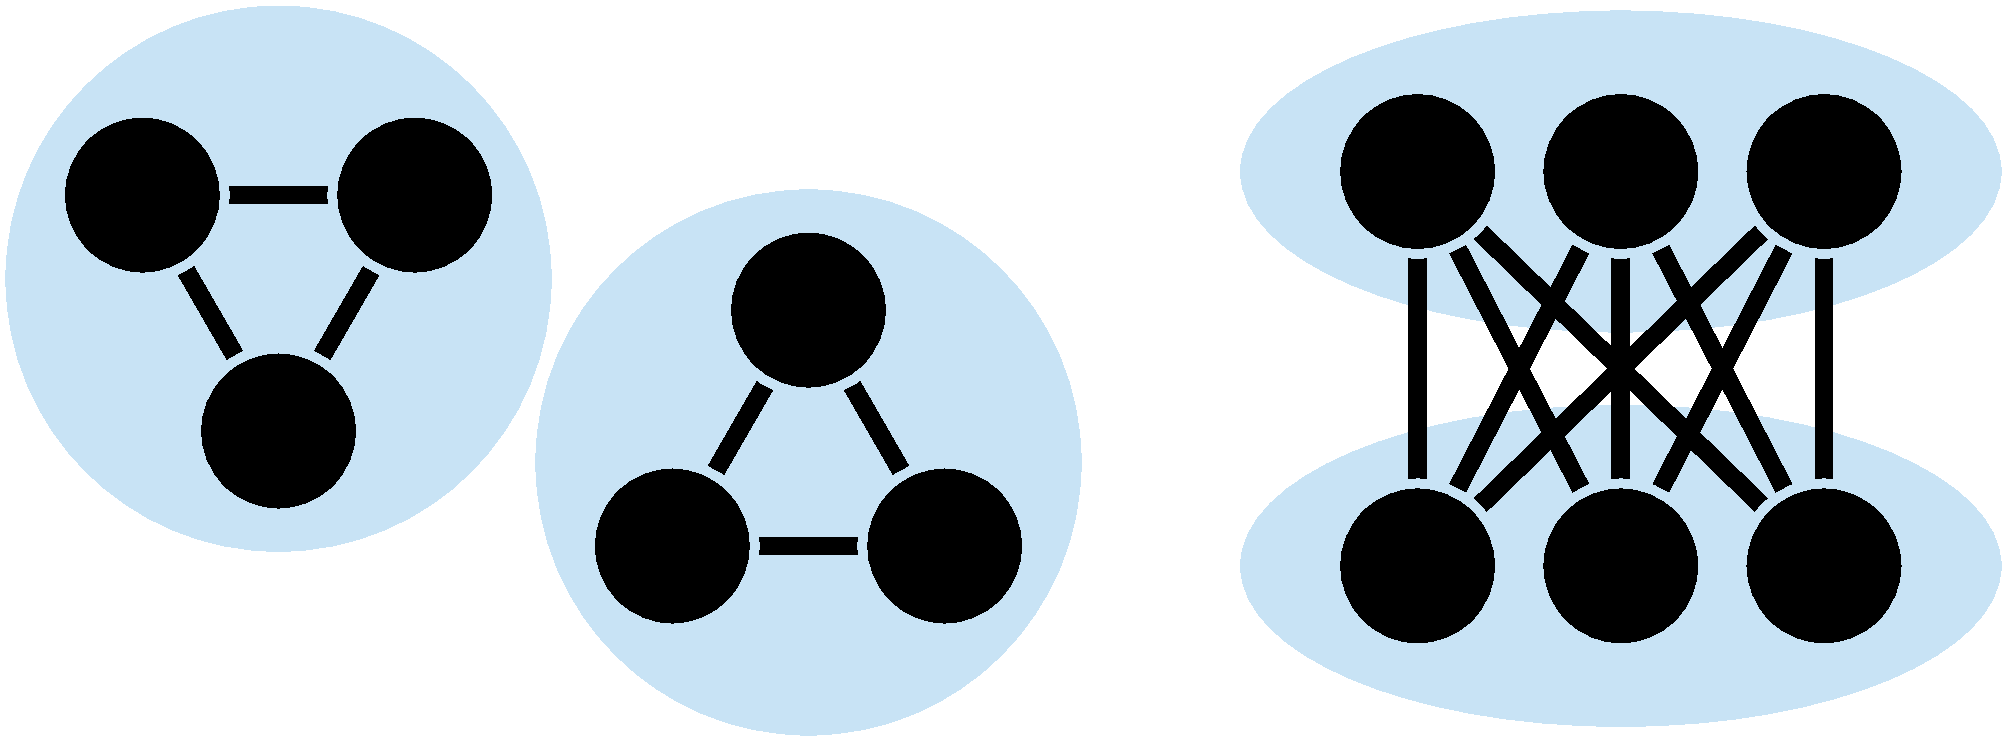
\includegraphics[width=.8\textwidth]{power/clique_vs_biclique.pdf}
  \caption[Two examples for why clustering is difficult to define]{An example of different types of clusters. On the left is a situation with edges within clusters, and on the right with edges between clusters.}
  \label{fig:clique_vs_biclique}
\end{figure}
It is therefore important to keep in mind that clustering algorithms are attempts to quantify common characteristics of real-world data, and there is generally no `right answer' to the question of which one should be chosen; it depends on both the specific objective and dataset being examined. 
Nevertheless, they have been used to great effect in many applications \cite{Fortunato2016}, and so confidence can be placed in their utility as a tool to help understand patterns in data.

The work in this chapter will focus on \emph{hierarchical clustering}, the family of clustering algorithms where the output is a \textit{dendrogram:} a binary tree used to describe a hierarchical structure.
This can either be done from the bottom up, i.e.\ each node starts in its own cluster and pairs of clusters are progressively merged until only one remains, or top down, i.e\ every node starts in the same cluster that is recursively split into two halves. The former is known as \emph{agglomerative} clustering, and the latter as \emph{divisive} clustering.
The output fits well here, since the goal is to construct a hierarchical edge bundling visualisation like the one in Figure~\ref{fig:metaunity}, but without a prior hierarchy included with the data; the dendrogram produced from such a clustering algorithm can be used as this missing hierarchy.

This idea of using the output dendrogram of a clustering algorithm to produce hierarchical edge bundling has been previously explored by Jia et al.\ \cite{Jia2011} who produce a hierarchy using the algorithm of Girvan and Newman \cite{Girvan2002}. This method removes one edge from the network at a time, specifically the one with the most \emph{betweenness centrality} i.e.\ the edge traversed the most often when mapping the shortest paths between all pairs of vertices. This naturally splits clusters when an edge is removed that is the final bridge between two clusters.
Unfortunately Jia et al.\ did not perform any quantitative analysis to evaluate the performance of their clustering algorithm, and only present results when using one clustering method. The work in the following section will aim to extend their work by evaluating the performance of a number of hierarchical clustering methods, against a benchmark of graphs where the ground truth cluster configuration is known.

\section{Hierarchical clustering}
\label{sec:hierarchical_clustering}
\begin{figure}
  \centering
  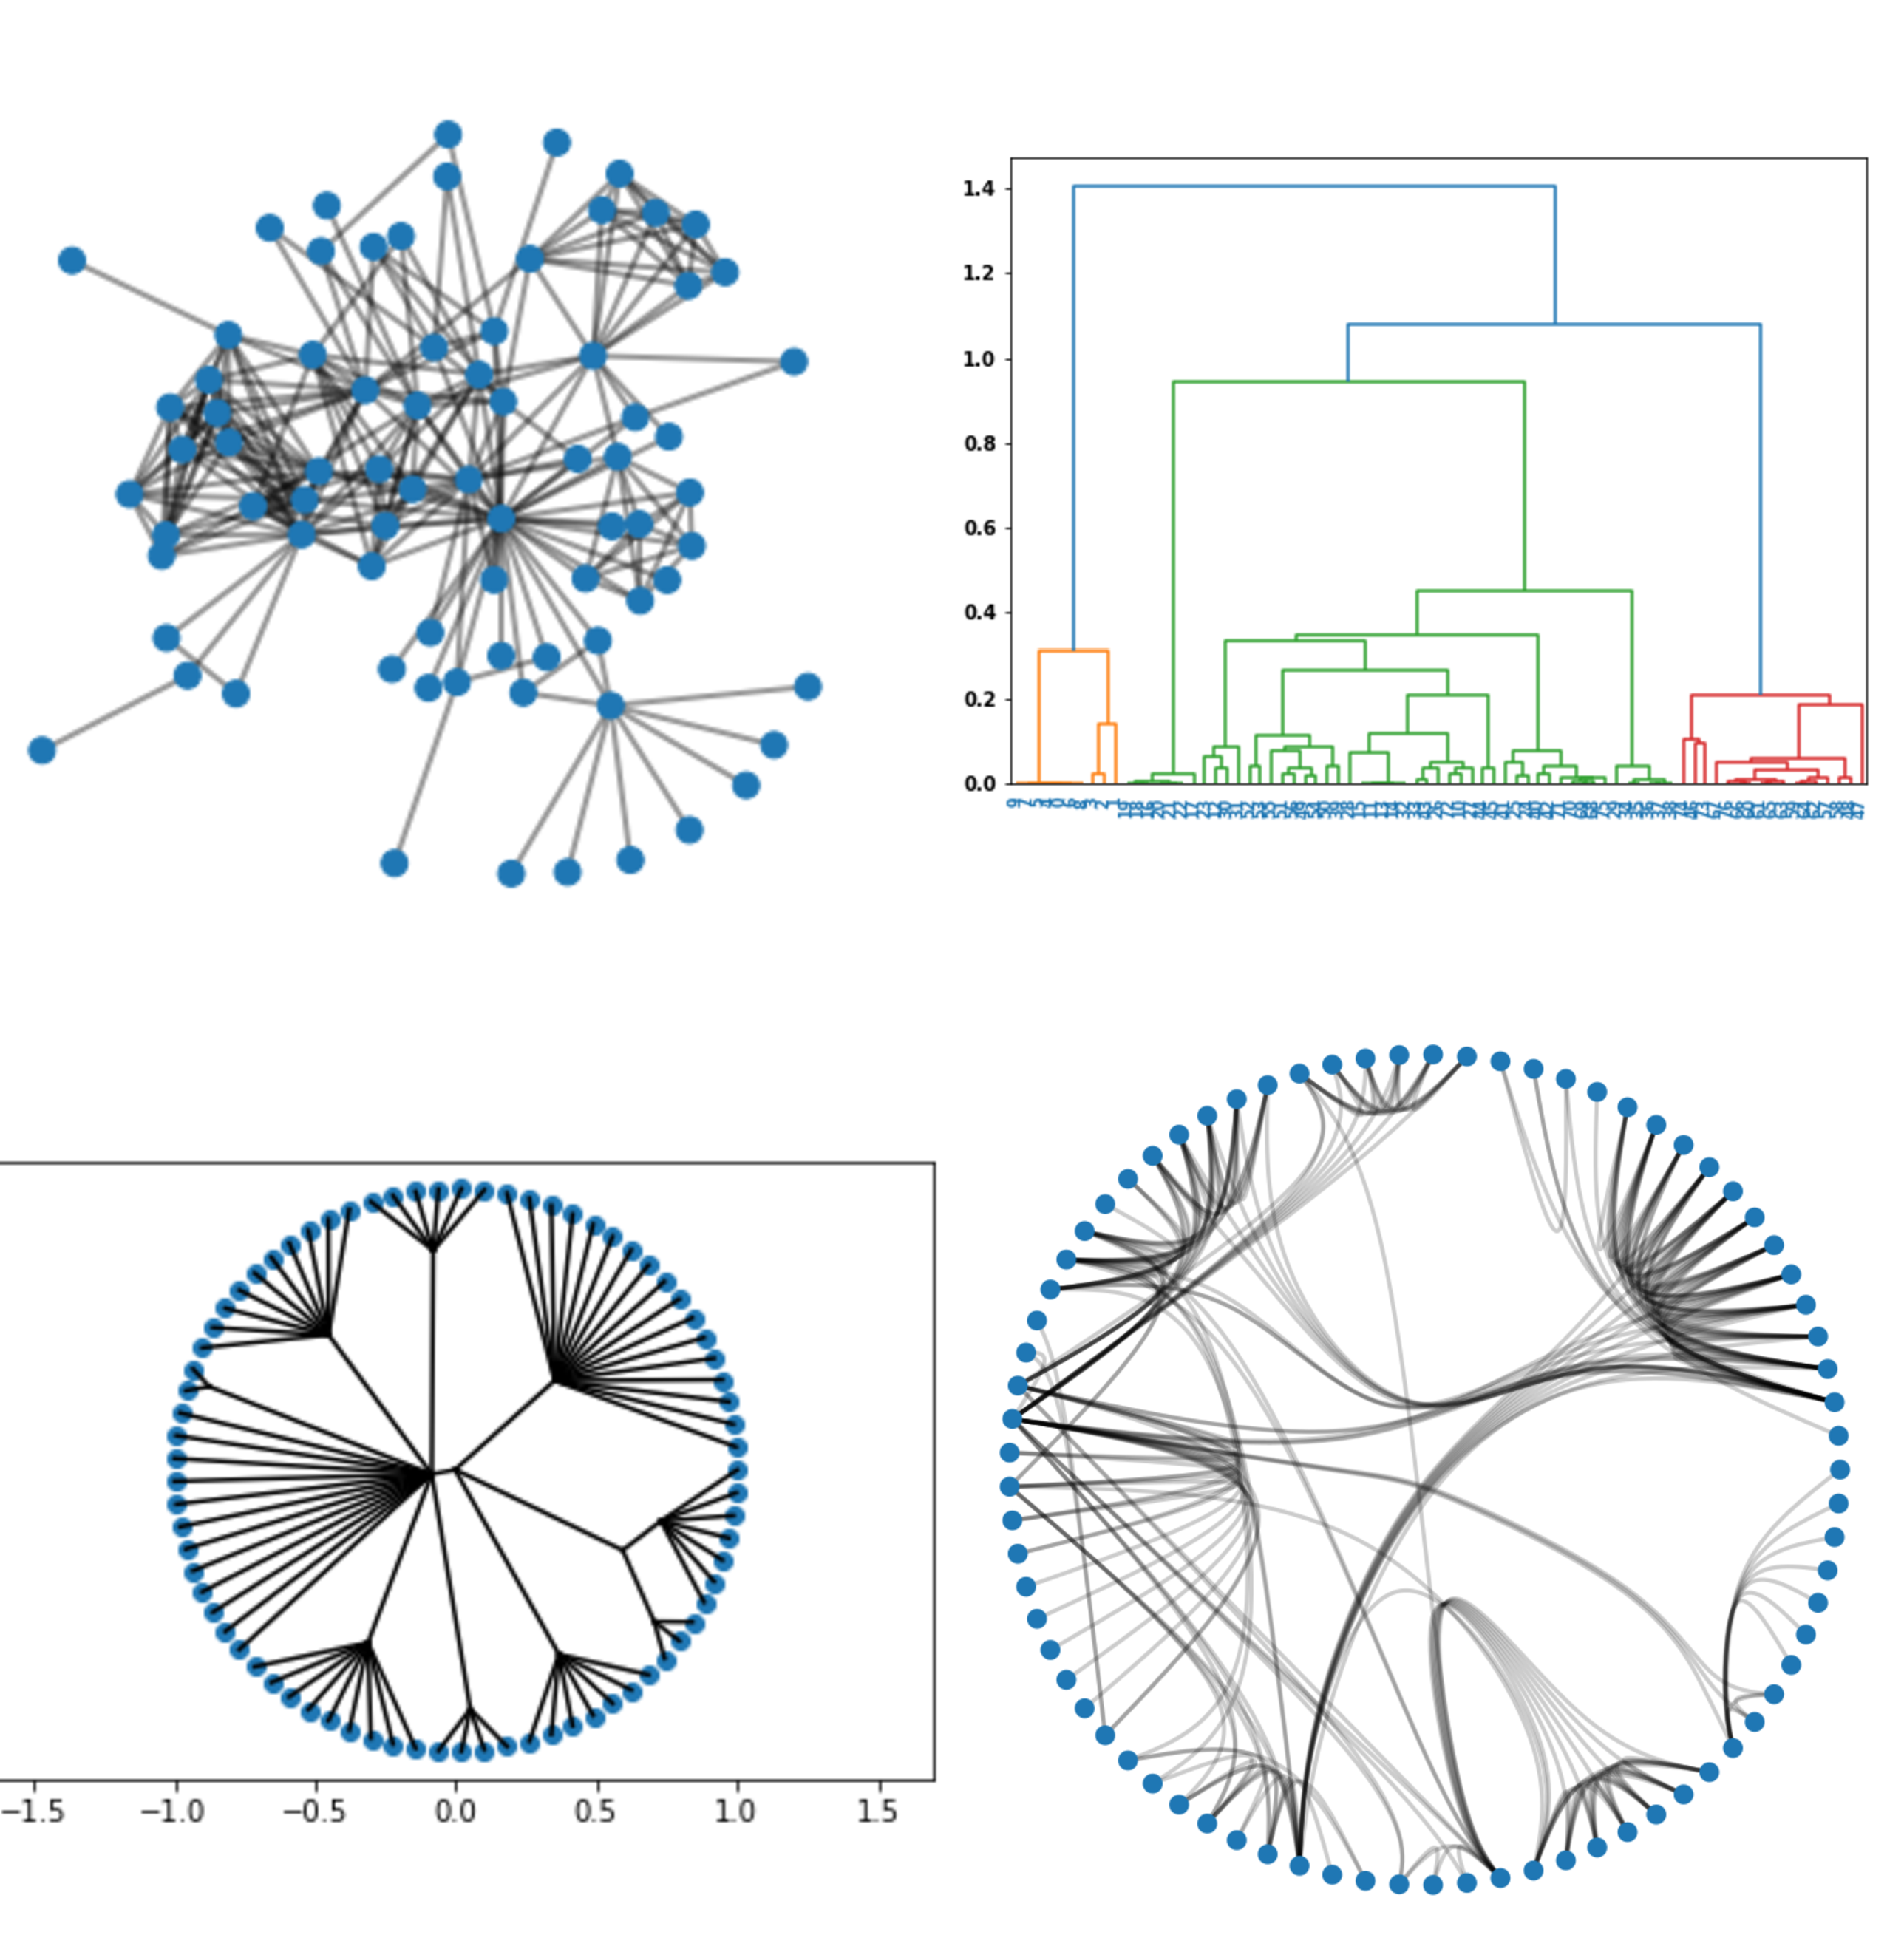
\includegraphics[width=\textwidth]{power/lesmis.pdf}
  \caption[A hierarchical edge bundling pipeline]{An example of the hierarchical edge bundling pipeline presented here, on the graph \texttt{lesmis} which describes co-appearances of characters in the musical les Mis\'erables \cite{Knuth1993}. The top-left is a layout from stress optimisation; top-right is a dendrogram computed from agglomerative dissimilarity clustering (see Section~\ref{sec:dissimilarities}); bottom-left is the tidied up hierarchical tree after pruning (see Section~\ref{sec:pruning}); bottom-right is the final hierarchical edge bundling diagram when original edges are rendered using splines (see Section~\ref{sec:heb_background}).
  The characters Jean Valjean and Javert are the main protagonist and antagonist respectively, and they are placed next to each other for both the stress and bundled layouts. Those two are highlighted, as well as a third main character, Marius, whose role in the network is much clearer in the bundled layout.}
  \label{fig:lesmis}
\end{figure}
To assess the quality of the divisive Girvan-Newman (GN) algorithm used by Jia et al.\ \cite{Jia2011}, it will be compared with \emph{agglomerative dissimilarity clustering}.
This is a family of algorithms where the input is a matrix of \emph{dissimilarities} between individual datapoints, in this case the vertices of a graph, and the output is a dendrogram as required. Similarly to the stress-based layout explored in the previous chapter, it is a more general algorithm that can be applied to any numerical datasets and not just graphs, unlike the methods previously outlined in Section~\ref{sec:clustering_background}. It is also closely related to the class of multidimensional scaling methods that stress minimisation belongs to, as both procedures take a matrix of dissimilarities as input.

Not only does this fit thematically with the topics explored in previous chapters, but a key benefit to using dissimilarity clustering is that the output dendrogram contains extra information to describe the `quality' of the merge at that point. This information is vital as it can be used to `prune' the hierarchical tree in order to make the resulting edge bundles more salient. This will be elaborated upon in Section~\ref{sec:pruning}, and an example of the method pipeline from start to finish is illustrated in Figure~\ref{fig:lesmis}.
Two other questions must first be answered before one can proceed with performing this clustering: what exactly are the dissimilarities to be used as input, and how will the algorithm proceed to process these dissimilarities to merge clusters? These will both be answered in the following section.

\subsection{Dissimiliarity clustering}
\label{sec:dissimilarities}
General hierarchical clustering based on dissimilarities can be done in both an agglomerative and divisive way, but the work here will focus on agglomerative methods. Agglomerative methods are more popular among practitioners \cite{Roux2018} due largely to the divisive version having $\mathcal{O}(2^{|V|})$ possible splits for a cluster of size $|V|$, as each datapoint can be placed in either one half or the other. This results in an exponential runtime complexity per split, whereas the agglomerative method has only to chose from pairs of datapoints, giving an $\mathcal{O}(|V|^2)$ complexity per merge.

There do exist heuristics to speed up the divisive method to bring the complexity down to polynomial, such as using algorithms like k-means to decide the split instead \cite{Lamrous2006}.
% It can also be argued that a divisive method can take a more global approach.
However, since there already exists a graph-specific divisive method in the GN algorithm to compare to, the work on this chapter will focus on comparing it to its agglomerative counterparts.

\subsubsection{Greedy agglomeration}
The agglomerative process is as follows:
\begin{mdframed}[backgroundcolor=WhiteSmoke]
\begin{enumerate}[leftmargin=*]
  \item Calculate the dissimilarities between all pairs of datapoints. \label{item:agglomerate_calculate}
  \item Place each datapoint into its own singleton cluster.
  \item Iterate over each pair of clusters, and merge the closest pair into a single cluster. \label{item:agglomerate_pairs}
  \item Recalculate the dissimilarities between the newly merged cluster and the remaining unmerged clusters. \label{item:agglomerate_recalculate}
  \item Repeat steps \ref{item:agglomerate_pairs} and \ref{item:agglomerate_recalculate} until only one supercluster remains.
\end{enumerate}
\end{mdframed}
On the surface this is a simple procedure, but it is not immediately clear how to calculate dissimilarities between datapoints or between clusters in steps \ref{item:agglomerate_calculate} or \ref{item:agglomerate_recalculate}.
There are an abundance of choices for what to use for step \ref{item:agglomerate_calculate}, which is the same first step as used in stress-minimisation from Section~\ref{sec:stress_background}. There, the graph-theoretic shortest-path was used as the dissimilarity, but there exist a wide variety of other measures that can be used that result in higher quality results. This will be shown in the experimental comparison in Section~\ref{sec:clustering_experiment} and discussed later in this section. Here The assumption that a dissimilarity is already defined between datapoints will first be taken, to begin by outlining how they are recalculated when clusters are merged.

There are also many choices for recalculating dissimilarities between clusters, and each choice can be thought of as a different heuristic for the greedy choice of which pair of clusters to merge together.
The most commonly used methods fall into three categories: using one member of a cluster as a representative, averaging over all cluster members, and measuring the variance of members within a cluster \cite{Roux2018}.
Choosing a single representative member is the most straightforward; when calculating the dissimilarity between two clusters, one can take the best-case scenario by choosing the closest pair of inter-cluster points, or the worst-case by choosing the farthest pair. These are known as single- and complete-linkage algorithms, respectively \cite{Sibson1973, Defays1977}.
One can also choose to take an average over the members of both clusters. This can be done by taking the mean dissimilarity between all inter-cluster pairs, and and is known as UPGMA (Unweighted Pair Group Method with Arithmetic mean). Its `weighted' counterpart, known as WPGMA, is more efficient, as when a cluster is merged it `forgets' that it was made up of other elements and becomes treated as a single datapoint itself \cite{Sneath1973}. The reason it is called weighted is, perhaps confusingly, because the original datapoints `lose weight' by being merged into a cluster, whereas in the unweighted version each original datapoint still contributes the same amount to each merging decision.

The third category is known as Ward's method \cite{WardJr1963}, and is based on minimising variance within clusters. The dissimilarity between clusters in this case is the increase in total within-cluster variance if they were to be merged. This is the same objective function that k-means clustering attempts to minimise \cite{Friedman2001Nearest}.
% \footnote{A good interpretation for the behaviour of different linkage methods is to imagine their shape. Single linkage is an amoeba absorbing the closest point around it, complete is a hypersphere expanding as little as possible, upgma b, wpgma, ward is a 'type' see \url{https://stats.stackexchange.com/questions/195456/how-to-select-a-clustering-method-how-to-validate-a-cluster-solution-to-warran/195481\#195481}}

Note that since each merge is based on the dissimilarity between clusters, this extra information that can be stored in the resulting dendrogram as the height of the branch. This is a direct benefit of using dissimilarity clustering, and is usually used to decide where to cut the dendrogram if flat clusters are needed. It will be leveraged to simplify the resulting dendrogram in Section~\ref{sec:pruning}.
However this is also a source of trouble for Ward's method specifically, because a monotonically increasing branch height is only guaranteed if the input is a \emph{distance}, and not just a \emph{dissimilarity}.
A distance must strictly satisfy the conditions
\begin{equation}
\begin{aligned}
  d_{ij} & \geq 0 \quad\text{and}\quad d_{ij}=0 \Leftrightarrow i=j \\
  d_{ij} & = d_{ji} \\
  d_{ij} & \leq d_{ik} + d_{ky}
\end{aligned}
\end{equation}
where the third condition is known as the triangle inequality, and is a requirement for the points to have a corresponding embedding in a metric space, such as Euclidean.
A dissimilarity is only required to satisfy the first two conditions.
Since Ward's method is based on variance, a concept that only makes geometric sense in a metric space, using a dissimilarity may result in dendrograms with negative branch lengths, making it impossible to cut the tree and form flat clusters.

The results in Section~\ref{sec:clustering_experiment} will include both distances and dissimilarities, both applied to Ward's method and the others reviewed in this section.
In practice, any reasonable dissimilarity does not often result in negative branch lengths with Ward's method, even if it does not satisfy the criteria of a distance. None of the results presented on the benchmark used here have this problem, but it is important to note the possibility of it happening in practice.

The final thing to discuss before moving onto how to choose a dissimilarity is the computational complexity on recalculating dissimilarities between clusters when they are merged. Remarkably, all of the above methods can be recalculated based on the Lance-Williams equation
\begin{equation}
  \;d_{\{i\cup j\}k} = \alpha_i d_{ik} + \alpha_j d_{jk} + \beta d_{ij} + \gamma|d_{ik}-d_{jk}|
  \label{eq:lancewilliams}
\end{equation}
where $d_{\{i\cup j\}k}$ is the new distance between $k$ and a newly merged cluster containing $i$ and $j$, and the values of $\alpha$, $\beta$, and $\gamma$ can all be calculated in constant time.
Recalculating the dissimilarity matrix after a merge therefore takes $\mathcal{O}(|V|)$ time. Searching through this matrix to find the best merge takes $\mathcal{O}(|V|^2)$ time, but this can be reduced to $\mathcal{O}(|V|\log(|V|)$ with a priority queue. Since forming a complete dendrogram requires $\mathcal{O}(|V|)$ merges, the overall complexity of greedy agglomerative clustering is $\mathcal{O}(|V|^2\log(|V|)$ .


\subsubsection{Random walks as dissimilarities}
The first step before performing the agglomeration is to calculate the pairwise dissimilarities between individual datapoints. As previously noted, the shortest path distance was used in the context of optimising stress, but it be shown here that this is far from optimal in a clustering context.
The reason for this that there is not enough \emph{local} information to differentiate vertices successfully.
For example, imagine a graph with two fully connected cliques, but with one edge connecting a single inter-cluster pair (one edge connecting the two clusters to the left of Figure~\ref{fig:clique_vs_biclique}). Since the shortest path between the pair is one hop, it means that the pair is considered just as similar to each other as to the other vertices in their respective cliques.
Similarly, vertices in the same group within a biclique are not connected at all (right side of Figure~\ref{fig:clique_vs_biclique}) and so within-cluster pairs would be considered even less similar than inter-cluster pairs.

A commonly used distance to capture local detail is the Jaccard index
\begin{equation}
  d_{ij} = 1 - \frac{|N(i) \cap N(j)|}{|N(i) \cup N(j)|}
  \label{eq:jaccard}
\end{equation}
which can be interpreted as the proportion of neighbours shared between vertices $i$ and $j$. However, this has the exact opposite problem to using shortest paths, as it fails to capture any \emph{global} detail, because any pair of vertices more than two hops away can never share any neighbours, and so will always have a maximum dissimilarity of one.
An ad hoc solution to this problem is to combine the two measures by simply multiplying them together, following Zheng et al.\ \cite{Zheng2018}. Note that despite shortest paths and Jaccard index both being distance metrics \cite{Clarkson2006}, it is not guaranteed the product of dissimilarities will also be.

A popular method of graph clustering that uses dissimilarities as input is the \emph{cluster walktrap} method of Pons and Latapy \cite{Pons2006}. They use \emph{random walks} to first construct a high-dimensional embedding of each vertex.
To construct the high-dimensional embedding, the \emph{Markov chain} transition matrix of the graph is calculated, defined as
\begin{equation}
  \mathbf{P} = \mathbf{D}^{-1} \mathbf{A}
\end{equation}
where $\mathbf{D}$ is a diagonal matrix of degrees, where the entries are the sum of the corresponding row in $\mathbf{A}$, which is the adjacency matrix of the graph that is not necessarily binary if edges have weights. $\mathbf{P}$ is essentially a normalised $\mathbf{A}$ where rows sum up to one.

However, this is not directly used as the high-dimensional embedding because of the same problem as the Jaccard coefficient in Equation~\eqref{eq:jaccard}, that is it only captures local detail. This matrix is therefore multiplied by itself a number of times in order to simulate a longer random walk. However, multiplying too many times results in a matrix converging to a state only dependent on the in-degree of each vertex \cite{Pons2006}, and so the length of the walk is left as an input parameter that should be set to an intermediate value.
The distance is defined as
\begin{equation}
  d_{ij} = \sqrt{\sum_{k}\frac{(\mathbf{P}_{ik}^t - \mathbf{P}_{jk}^t)^2}{\mathbf{D}_{kk}}}
  \label{eq:walktrap}
\end{equation}
where $t>0$ is an input parameter that determines how many times $\mathbf{P}$ should be multiplied by itself.
Notice that this is very close to being simply the Euclidean distance between columns in $\mathbf{P}$, except with a factor consisting of $\mathbf{D}_{kk}^{\text{--}\sfrac{1}{2}}$. This was done presumably in order to undercompensate for high-degree vertices, although they state that their distance \textit{``can also be seen as the $L^2$ distance between the two probability distributions"} \cite{Pons2006} without mentioning this factor. However a look into their provided source code confirms the use of the factor.
Since this measure can also be written as the Euclidean distance between columns in the matrix $\mathbf{D}^{\text{--}\sfrac{1}{2}}\mathbf{P}^t$, it automatically also qualifies as a distance metric.
\cite{Pons2006} did not study whether the inclusion of this factor performs better quantitatively, and the performance on the benchmark used in Section~\ref{sec:clustering_experiment} is in fact always higher when this factor is left out. Equation~\eqref{eq:walktrap} will therefore be used without including it, i.e.\ simply $\sqrt{\sum_{k}(\mathbf{P}_{ik}^t - \mathbf{P}_{jk}^t)^2}$. This will be referred to as the \emph{snapshot} embedding, as it captures the random walker state after a fixed number of steps $t$.

The algorithm then proceeds by applying agglomerative clustering using the Ward method, but with one difference: it only merges clusters connected by an edge. This reduces computation time and likely improves the modularity of the resulting clusters, but since the end goal is to produce bundles, edges between clusters are acceptable as they will be bundled. The results here will therefore use the more general algorithm that is unaware of edges between clusters.

It is also not necessary to be restricted to having the embedding capture the random walker at a single walk length. Another type of embedding that will be used is the weighted average over all walk lengths. However this would also converge to the same matrix as an infinite length walk, by virtue of the Markov matrix converging to only depend on in-degrees as previously mentioned. In this case a \emph{damping factor} is used, similar to the one used in PageRank \cite{Page1999} and infomap clustering \cite{Rosvall2008} to simulate a random walker losing a proportion of its energy on each step and eventually coming to a stop. This is defined as
\begin{equation}
  \mathbf{P}' = \sum_{k=0}^\infty t^k\mathbf{P}^{k}
  \label{eq:damped}
\end{equation}
where $0<t\leq 1$ is an input parameter to represent the proportion of walkers that move on to take another step. This will be referred to as the \emph{damped} embedding, as it captures the random walker state damped over a range of step lengths. A range of values for $t$ from Equation~\eqref{eq:walktrap} will be systematically tested in the Section~\ref{sec:clustering_experiment}.

Random walks have many nice properties, including the 
an extra benefit of interpreting heavier edge weights as bringing vertices closer rather than farther away, as would be done in a standard shortest paths algorithm. This is more common in real world datasets, for example in a social network where an edge weight could indicate the frequency of two friends messaging each other, or in a food web where to indicate the strength of an interaction between two species.
The weights on the graph in Figure~\ref{fig:lesmis} describe how many times characters appeared in the same scene together, and this extra information was used in the clustering process.
The fact that the Markov chain matrix is a probability distribution also allows it to naturally be applied to measures such as the Kullback-Leibler (KL) divergence 
\begin{equation}
  d_{ij} = \sum_k \mathbf{P}_{ik}\log\left(\frac{\mathbf{P}_{ik}}{\mathbf{P}_{jk}}\right)
  \label{eq:kullbackleibler}
\end{equation}
which can be interpreted as the relative entropy of $i$ relative to $j$.
Another popular measure is the Wasserstein distance
\begin{equation}
  d_{ij} = \int_{-\infty}^{\infty}|\mathbf{F}(i) - \mathbf{F}(j)|
\end{equation}
where $\mathbf{F}_i$ denotes the cumulative probability distributions of $i$ and $j$ \cite{Ramdas2017}. This can be interpreted by imagining the area under the curve of one distribution as mass to be moved, and measuring the amount of work needed to transform that mass into the second distribution.
Both are natural and popular dissimilarities in the context of probability that are commonly used in the field of machine learning \cite{Goodfellow2014, Arjovsky2017}. The Wasserstein distance is already a distance metric \cite{Villani2003} and so can safely be used as an input. KL is not even a dissimilarity in Equation~\ref{eq:kullbackleibler} as it is not symmetric, and so it is commonly symmetrised by adding the two directions together as $d'_{ij} = d_{ij} + d_{ji}$ \cite{Kullback1951}.
 
One final dissimilarity based on random walks that has been applied before to clustering applications is the Euclidean commute time distance \cite{Yen2005}. This is defined as the average time it takes for a random walker to travel from a one vertex to the other and then back again.
It is also a distance metric \cite{Qiu2007}, and can be found in closed form using the Moore-Penrose pseudoinverse of the Laplacian matrix $\mathbf{L} = \mathbf{D}-\mathbf{A}$ as
\begin{equation}
d_{ij} = |E|(\mathbf{L}_{ii}^+ + \mathbf{L}_{jj}^+ - 2\mathbf{L}_{ij}^+)
\label{eq:commute}
\end{equation}
where $\mathbf{L}^+$ is the pseudoinverse of $\mathbf{L}$ \cite{Albano2012}.
% say laplacian is kirchoff for commute distance
The distances derived from Equations~\eqref{eq:jaccard}--\eqref{eq:commute} will all be used in the following section as part of an experimental study to determine which is most effective.

\subsection{Experimental study}
\label{sec:clustering_experiment}
Since clustering is an undefined problem, the quality of clusters will be measured by using a benchmark set of graphs where a ground truth clustering configuration is known.

Table~\ref{tab:bundle_graphs} contains the four graphs used in this study.
The graph \texttt{karate} is a classic dataset that has been extensively studied in the network research literature \cite{Fortunato2016}, originally compiled by Zachary \cite{Zachary1977}. It is a social network containing relationships between members of a karate club, in which a rift between two club leaders caused the club to split into two new clubs, where the resulting members of the two clubs form the ground truth clustering of the data.
The \texttt{footballTSE} graph is a network of American football games between Colleges in the US, where the ground truth is the conference in which they belong. It was originally studied by Girvan and Newman \cite{Girvan2002} in the same paper as the GN algorithm was presented. The ground truth data used is a version corrected by Evans \cite{Evans2010}, as the original data clusters were assigned from the 2001 season instead of the correct 2000 season. 
The \texttt{caltech} graph is a social network of students at the California Institute of Technology, extracted from the website Facebook and originally studied by Traud et al.\ \cite{Traud2012}. It has been shown to demonstrate clique structure \cite{Nocaj2015}, where the ground truth used here are the dorms in which students were living. This is the most messy data and so the dorm ground truth is the least well matched by the clustering algorithms used.
% The original graph contains 769 vertices, so the largest connected component was used here.
The \texttt{lfr} graph is a sample graph from the Lancichinetti Fortunato Radicchi (LFR) benchmark \cite{Lancichinetti2008} which is a model to generate graphs with a clustered structure, given a number of parameters to account for power law distributions in cluster size and vertex degree. The parameters used here were $\tau_1=3$, $\tau_2=1.5$, and $\mu=0.1$. They represent the degree distribution, community size, and fraction of edges to place between communities, respectively. The LFR benchmark was developed in order to improve the popular random model of Girvan and Newman \cite{Girvan2002}.
%In practice the \texttt{networkx} implementation is not very robust to changes in parameters $\alpha=?$
All graphs are undirected and unweighted.

\begin{table}
  \centering
  \caption[Benchmark graphs used for the experiment in Section~\ref{sec:clustering_experiment}]{Benchmark graphs used for the experiment in Section~\ref{sec:clustering_experiment}. $|V|$ denotes the number of vertices, $|E|$ the number of edges, and $|M|$ the number of ground truth clusters.}
  \setlength{\tabcolsep}{1em} % for the horizontal padding
  {\renewcommand{\arraystretch}{1.25}% for the vertical padding
  \begin{tabular}{|c|c|c|c|}
    \hline
    Name & $|V|$ & $|E|$ & $|M|$
    \\\hline\hline
    \texttt{karate} & 34 & 78 & 2
    \\\hline
    \texttt{footballTSE} & 115 & 613 & 19
    \\\hline
    \texttt{caltech} & 762 & 16651 & 9
    \\\hline
    \texttt{lfr} & 250 & 472 & 10
    \\\hline
  \end{tabular}}
  \label{tab:bundle_graphs}
\end{table}


These four graphs were run through each of the agglomerative methods presented in Section~\ref{sec:dissimilarities}. For methods that first require a high dimensional embedding, a range of parameters were used for the values of $t$ for Equations~\eqref{eq:walktrap} and~\eqref{eq:damped}.
To assess the quality of the results, the adjusted random index (ARI) was used to compare a ground truth clustering against the clusters predicted by the algorithm. The benefit of using ARI is that it is robust to cluster labels being swapped, avoiding the situation where the clusters are correct but the order of labels is not.
ARI is bounded between --$1$ and $1$, where a value of $1$ denotes perfect clustering, $0$ denotes a randomly shuffled clustering, and --$1$ denotes an even worse match than the expected result of a shuffle.
A problem with hierarchical clustering is that, to extract flat clusters to match the ground truth, the resulting dendrogram must be cut. The results here give the benefit of the doubt by measuring ARI at all cutting points and taking the maximum ARI of all cuts, to essentially assume that the algorithm always chooses its cut perfectly.

The package \texttt{scipy.cluster.hierarchy} \cite{Virtanen2020} was used to perform all hierarchical dissimilarity-based clustering.
Results are presented in Figures~\ref{fig:ARI1} and~\ref{fig:ARI2}, where all dissimilarity measures are clustered with each of the five linkage methods presented in Section~\ref{sec:dissimilarities}.

\begin{figure}
  \centering
  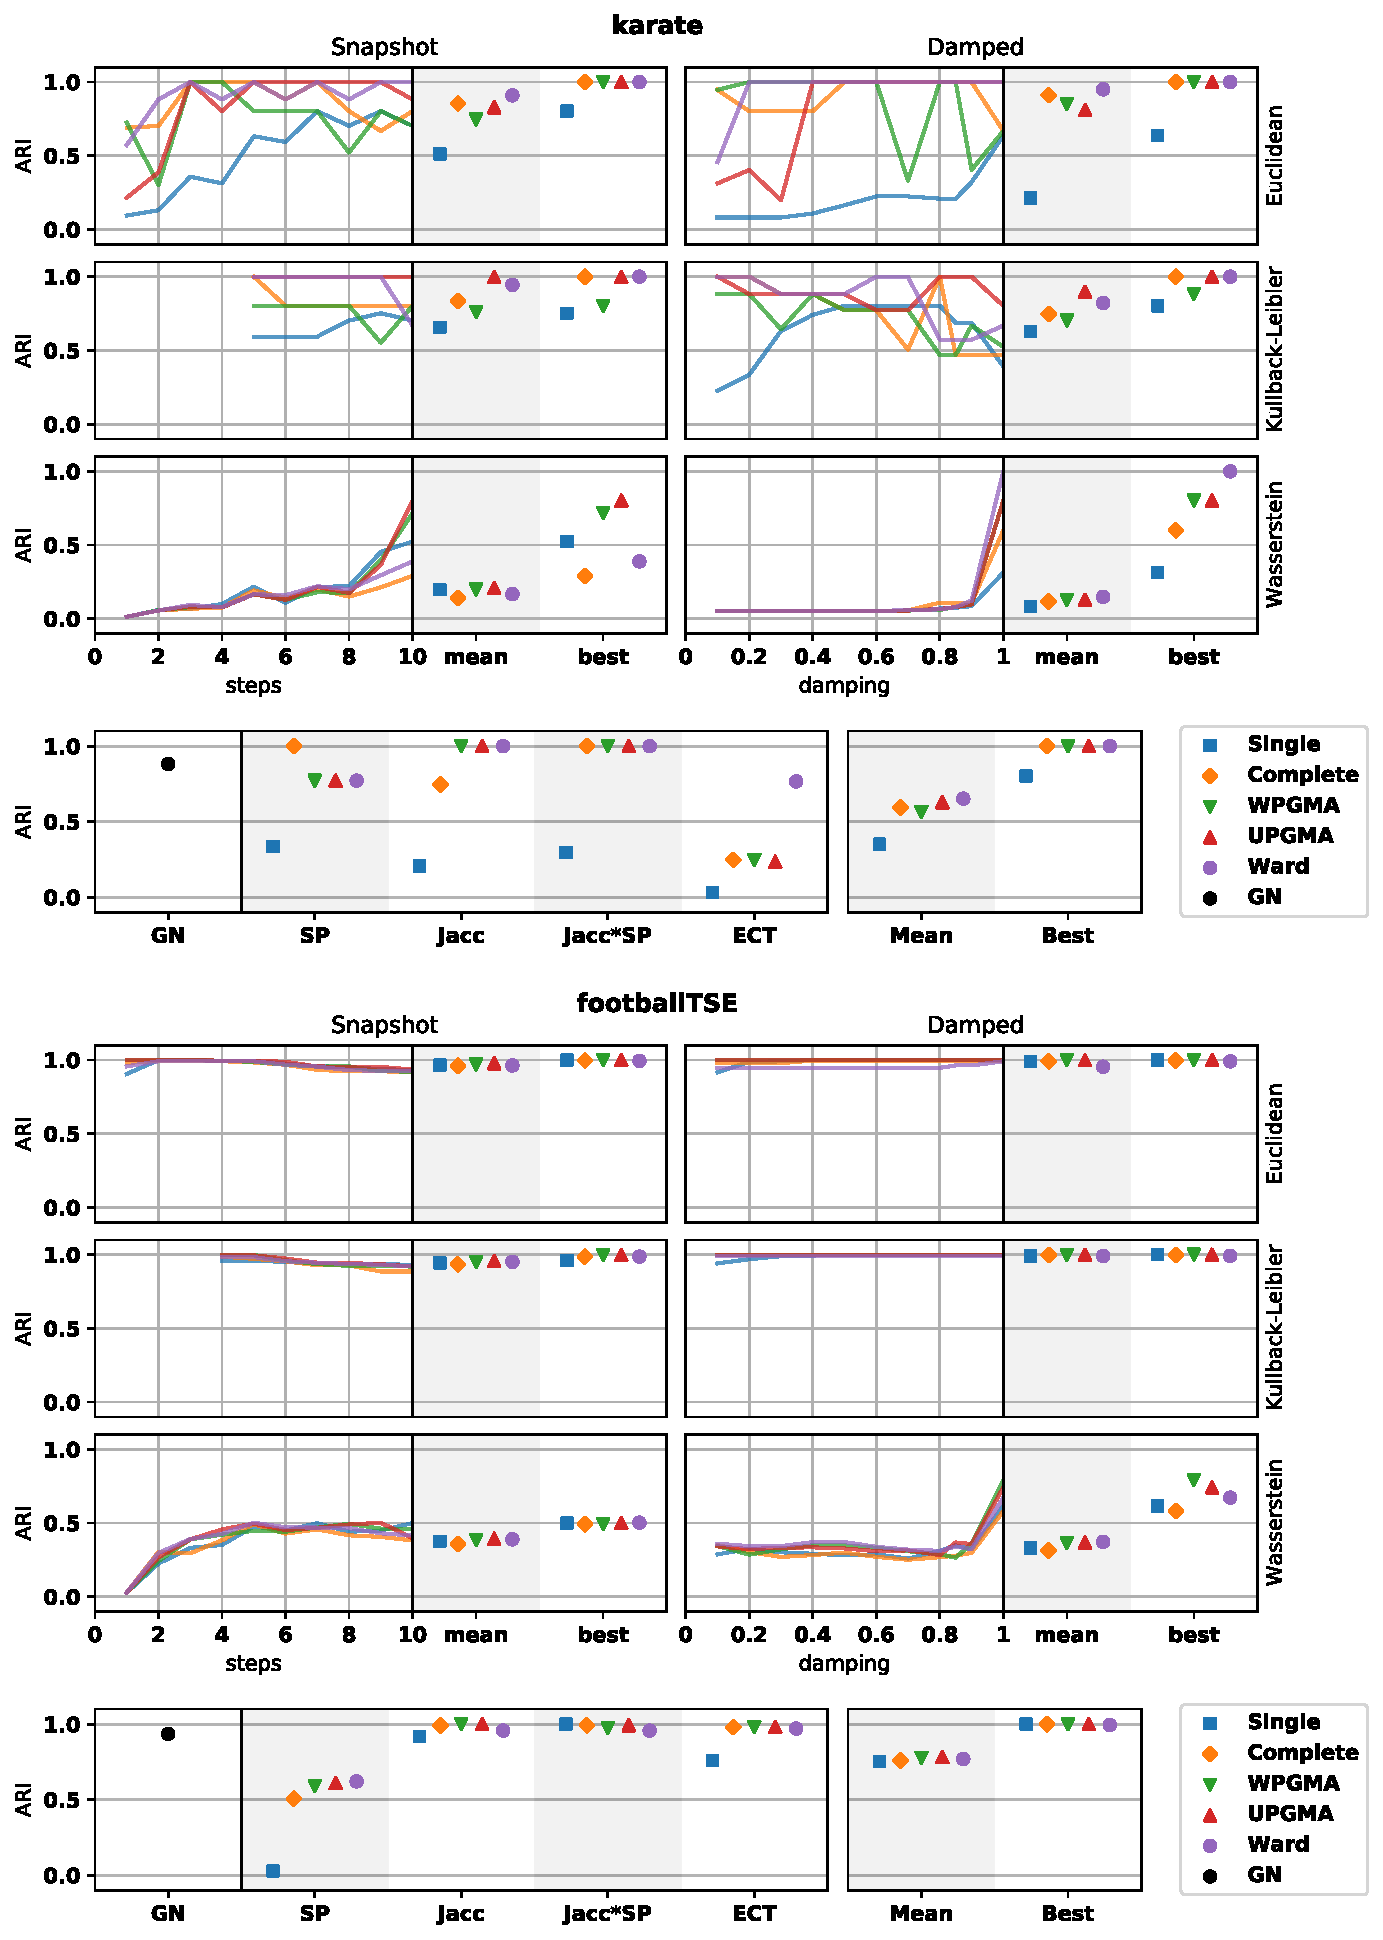
\includegraphics[height=.95\textheight]{power/ARI1.pdf}
  \caption[Experimental clustering results for \texttt{karate} and \texttt{footballTSE}]{Clustering performance on the graphs \texttt{karate} and \texttt{footballTSE}. Each linkage method is denoted by a different color and symbol.
  ARI is on y-axis, clustering algorithms on the x-axis.
  Average and best ARI over all clusterings is in bottom right. Missing values for KL are due to probabilities of 0 in the Markov chain.}
  \label{fig:ARI1}
\end{figure}
\begin{figure}
  \centering
  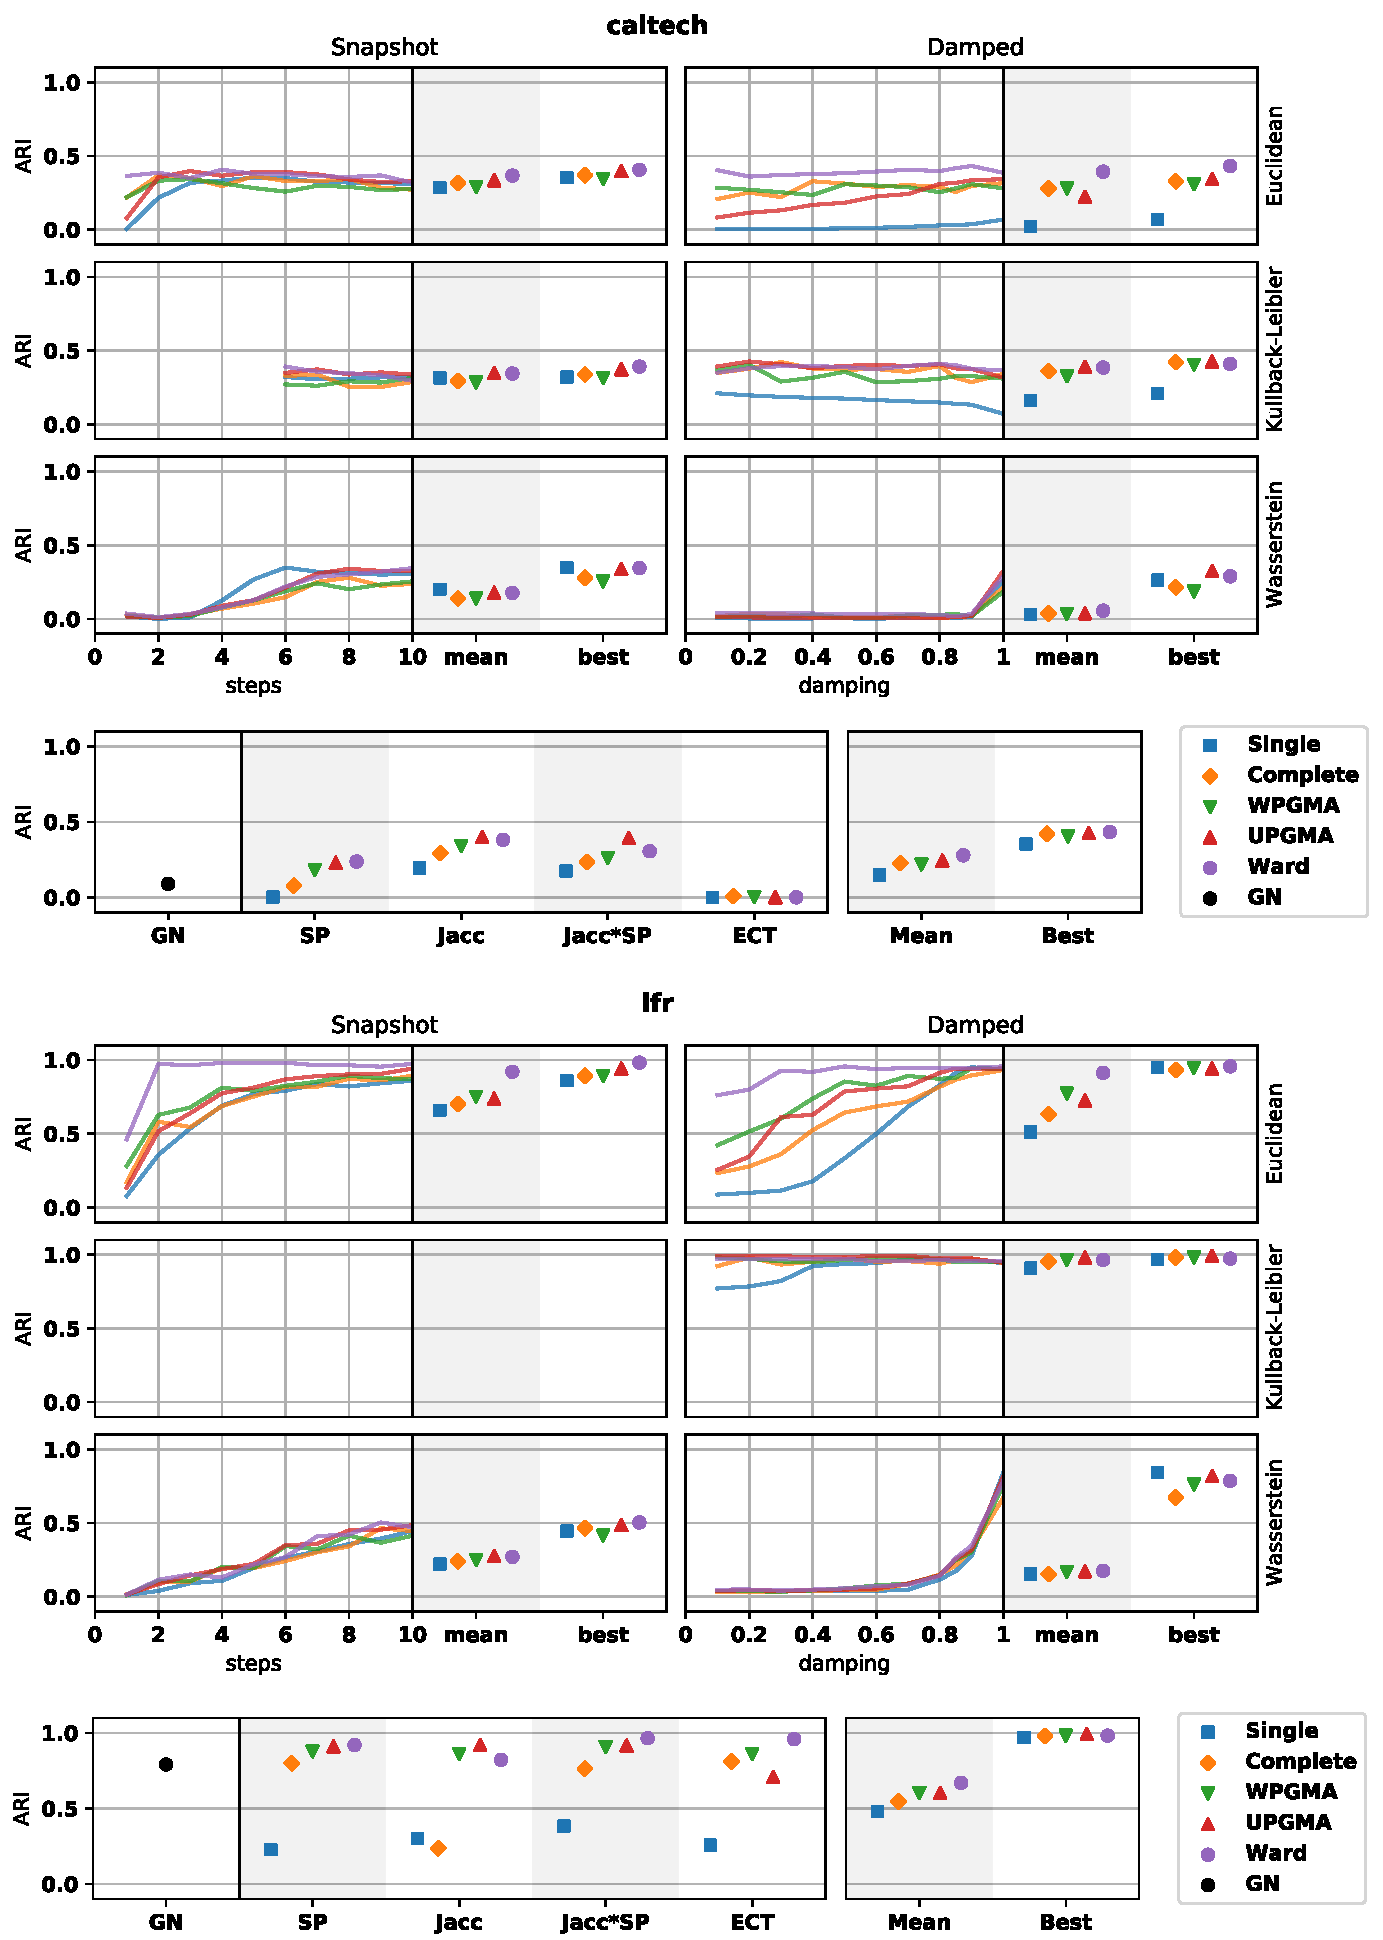
\includegraphics[height=.95\textheight]{power/ARI2.pdf}
  \caption[Experimental clustering results for \texttt{caltech} and \texttt{lfr}]{Clustering performance on the graphs \texttt{caltech} and \texttt{lfr}, following the same format as Figure~\ref{fig:ARI1}.}
  \label{fig:ARI2}
\end{figure}

\subsubsection{Results}
The aim of this study is to answer two questions: which dissimilarity measure is best, and which linkage method is best for clustering this dissimilarity?
Unfortunately there is no clear-cut answer to either question, but the results can be interpreted to give some recommendations. Looking at the bottom right panels for each graph, it is immediately clear that single linkage is the least effective and should be avoided. The best scores for the remaining linkage methods generally hover around the same value, and so it is clear that the remaining four linkage methods all \emph{can} result in high quality results. Looking at the mean ARI scores, however, it becomes apparent that Ward's method produces the best results on average. This is consistent with the choice made by Pons and Latapy \cite{Pons2006} for their clustering method, now with quantitative results to verify the decision.

% A more qualitative observation is that Ward also tends to give the best hierarchical structure in terms of neat trees without branches that, which is difficult to measure but results in the best bundles.
The best dissimilarity for Ward over all graphs is Euclidean on snapshot embedding with $t=5$ in Equation~\eqref{eq:walktrap}, and it seems the original authors in \cite{Pons2006} agree with this choice too, as they performed their analysis using either $t=2$ or $t=5$.
Using Equation~\ref{eq:damped} to take a weighted average of step lengths also does not improve the clustering performance, further confirming their design choices.
Despite being a distance metric, the performance of Wasserstein is consistently poorer than both Euclidean and KL. It is however worth noting that it consistently improves as the value of $t$ rises for both snapshot and damped embeddings. Both sets of parameters converge to the same embedding (the stationary distribution of the Markov chain) for $t\rightarrow \infty$ and $t\rightarrow 1$, respectively, so it seems that Wasserstein is effective on this stationary distribution, at least on this benchmark.

The alternative dissimilarities in the bottom left panels do not reach the same best values as the embeddings do, but they possess the important benefit not not needing to tune an extra parameter $t$, which is of great importance to practitioners. This is especially true given the variance of some of the lines in the top plots in Figures~\ref{fig:ARI1} and ~\ref{fig:ARI2}.
The Jaccard index combined with UPGMA consistently scored high in each of the test graphs, and so is also worth a recommendation as an interpretable and robust choice.
The remaining results in this chapter will use Ward's method on Euclidean distance over a snapshot embedding with $t=5$, due to the reasons outlined above.

\subsection{Pruning}
\label{sec:pruning}
The final step to producing a hierarchical edge bundling visualisation is to convert the resulting dendrogram into an edge bundled diagram. This is done by first laying out the hierarchy as a tree, and then redrawing the original edges back on top as splines routed up and down the hierarchy.
However a problem with using a dendrogram is that, as a binary tree, it contains as many branch nodes as leaves, which means that the resulting splines end up being routed through too many control points to separate individual edges. See Figure~\ref{fig:pruning} for an example of this on the \texttt{lesmis} graph.
The process of tidying up this tree such that it is suitable for use in hierarchical bundling will be referred to as \emph{pruning}. 

\begin{figure}
  \centering
  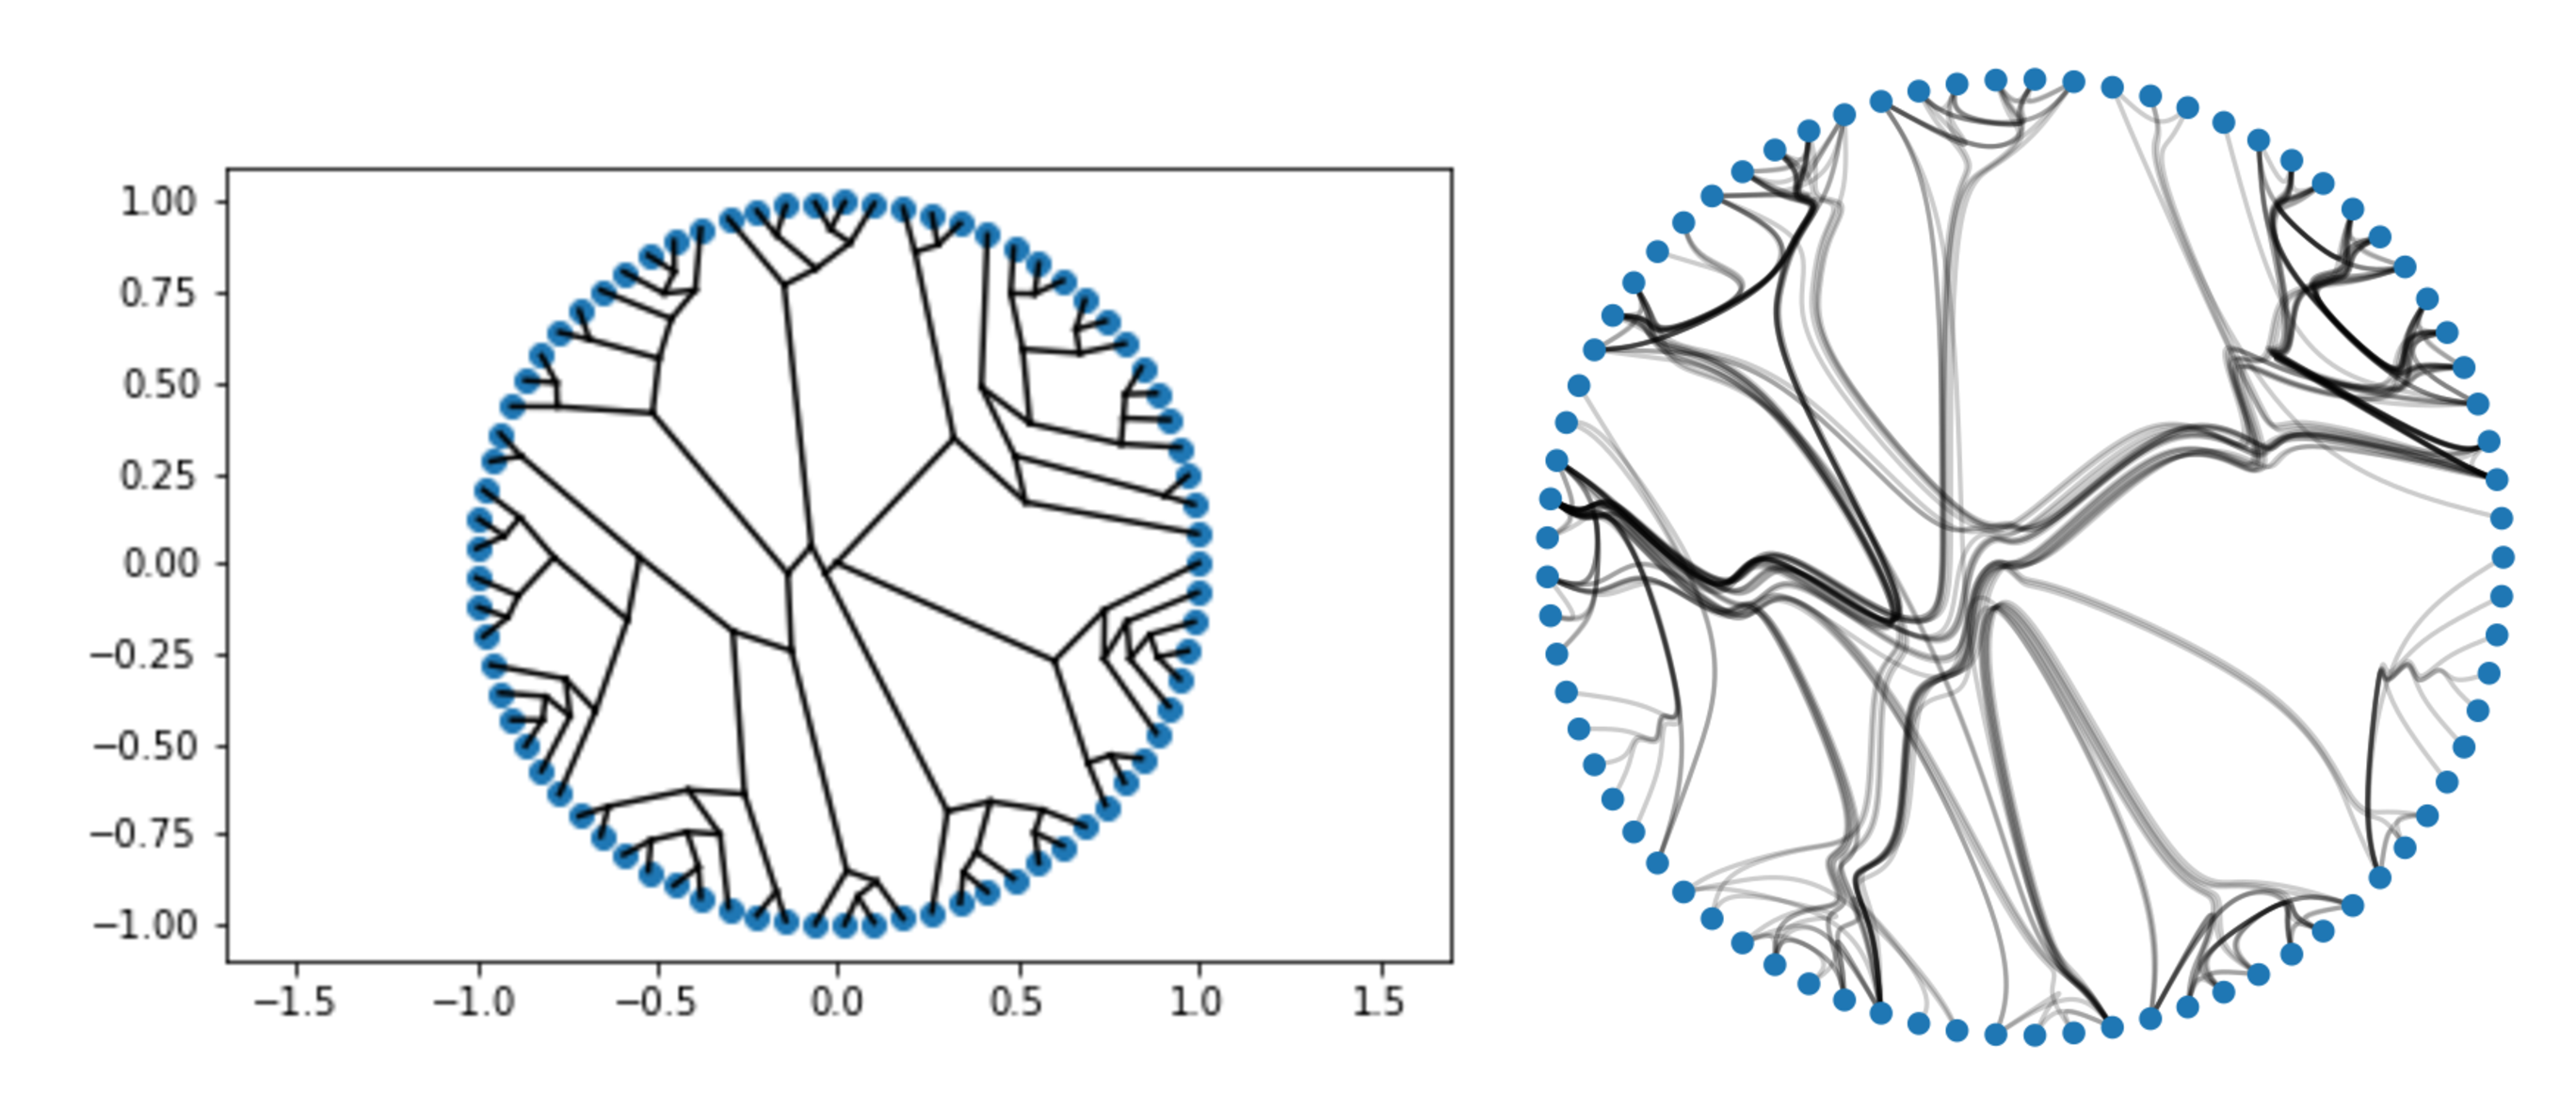
\includegraphics[width=.9\textwidth]{power/pruning.pdf}
  \caption[Hierarchical edge bundles without pruning]{An example of the resulting hierarchical edge bundles when pruning is not applied to the hierarchy. On the left is the full hierarchical dendrogram without pruning, and on the right is the resulting bundled diagram, which is clearly worse than the one in Figure~\ref{fig:lesmis}.}
  \label{fig:pruning}   
\end{figure}

Jia et al.\ \cite{Jia2011} also encountered the same problem when producing their hierarchical bundles using the resulting dendrogram from the GN algorithm. They alleviate this issue by applying a branch-merging procedure that leverages the fact that each branch corresponds to a disconnected subgraph, due to the progressive removal of edges at each step in the algorithm.
This cannot be applied to a general dendrogram, and so another property of dissimilarity clustering is used instead: the fact that each parent cluster can store the dissimilarity between its two child clusters before the merge. This is usually thought of as the height of each branch in the dendogram, as shown in the top-right of Figure~\ref{fig:lesmis}, and is used here to recursively merge branches in the hierarchy if their height difference falls below a certain threshold. This follows another similar idea of Pons and Latapy \cite{Pons2006} who use the same branch height information to determine an optimal cutting point for forming flat clusters.

The next step is to lay out the hierarchy itself as a tree. Following Holten \cite{Holten2006}, a radial tree layout is chosen, and since each leaf of the tree represents a vertex of the original graph, they are first placed around the circumference of the circle. The order in which leaves are placed around the circle is very important, as it directly affects the proximity of edges to be bundled together. This is a similar problem to seriation in matrix plots \cite{Liiv2010}.
Obviously any cousin vertices in the tree should be placed next to each other, but this still leaves an exponential number of orderings because the order within groups of cousins is still undecided.
Fortunately, a neat solution exists to this problem, as there exists an algorithm that can find an optimal ordering. The definition of optimal in this case is to minimise the total dissimilarity between leaves ordered next to each other.
Remarkably, this can be computed in polynomial time using the algorithm of Bar-Joseph et al.\ \cite{Bar-Joseph2001}, which leverages the structure of the hierarchical dendrogram to formulate the task as a dynamic programming problem. All resulting layouts presented here use this optimal ordering, although its complexity of $\mathcal{O}(|V|^4)$ makes it prohibitively slow for datasets any larger than the graphs studied here.
% This would not be applicable without a dendrogram, and so is another benefit of a hierarchical methodology.

The next step is to position the branches of the tree. Many methods were tested for determining branch placement, including the use of force-directed methods such as Tutte's algorithm as in Figure~\ref{fig:misc_force_layouts}, but the method settled upon was to use polar coordinates, in the following manner.
The angle of a parent is set to the mean of the angles of its children, and its distance from center is set proportional to the total number of leaves below it in the hierarchy. This means that the height of a branch corresponds to the size of its corresponding cluster, which is extra information embedded in the final visualisation.

The final step is to render the bundles itself. With the tree layout determined, this step is exactly the same as that of Holten \cite{Holten2006}. Important subtleties include relaxing bundles to prevent splines from overlapping too much, and skipping the lowest common ancestor as a control point in order to reduce clutter around common parent nodes.
The resulting visualisations for the four benchmark graphs in Table~\ref{tab:bundle_graphs} can be seen in Figure~\ref{fig:untangled_hairballs}.
Code used to generate all figures can be found at \url{www.github.com/jxz12/HierarchicalEdgeBundles}. 

\begin{figure}
  \centering
  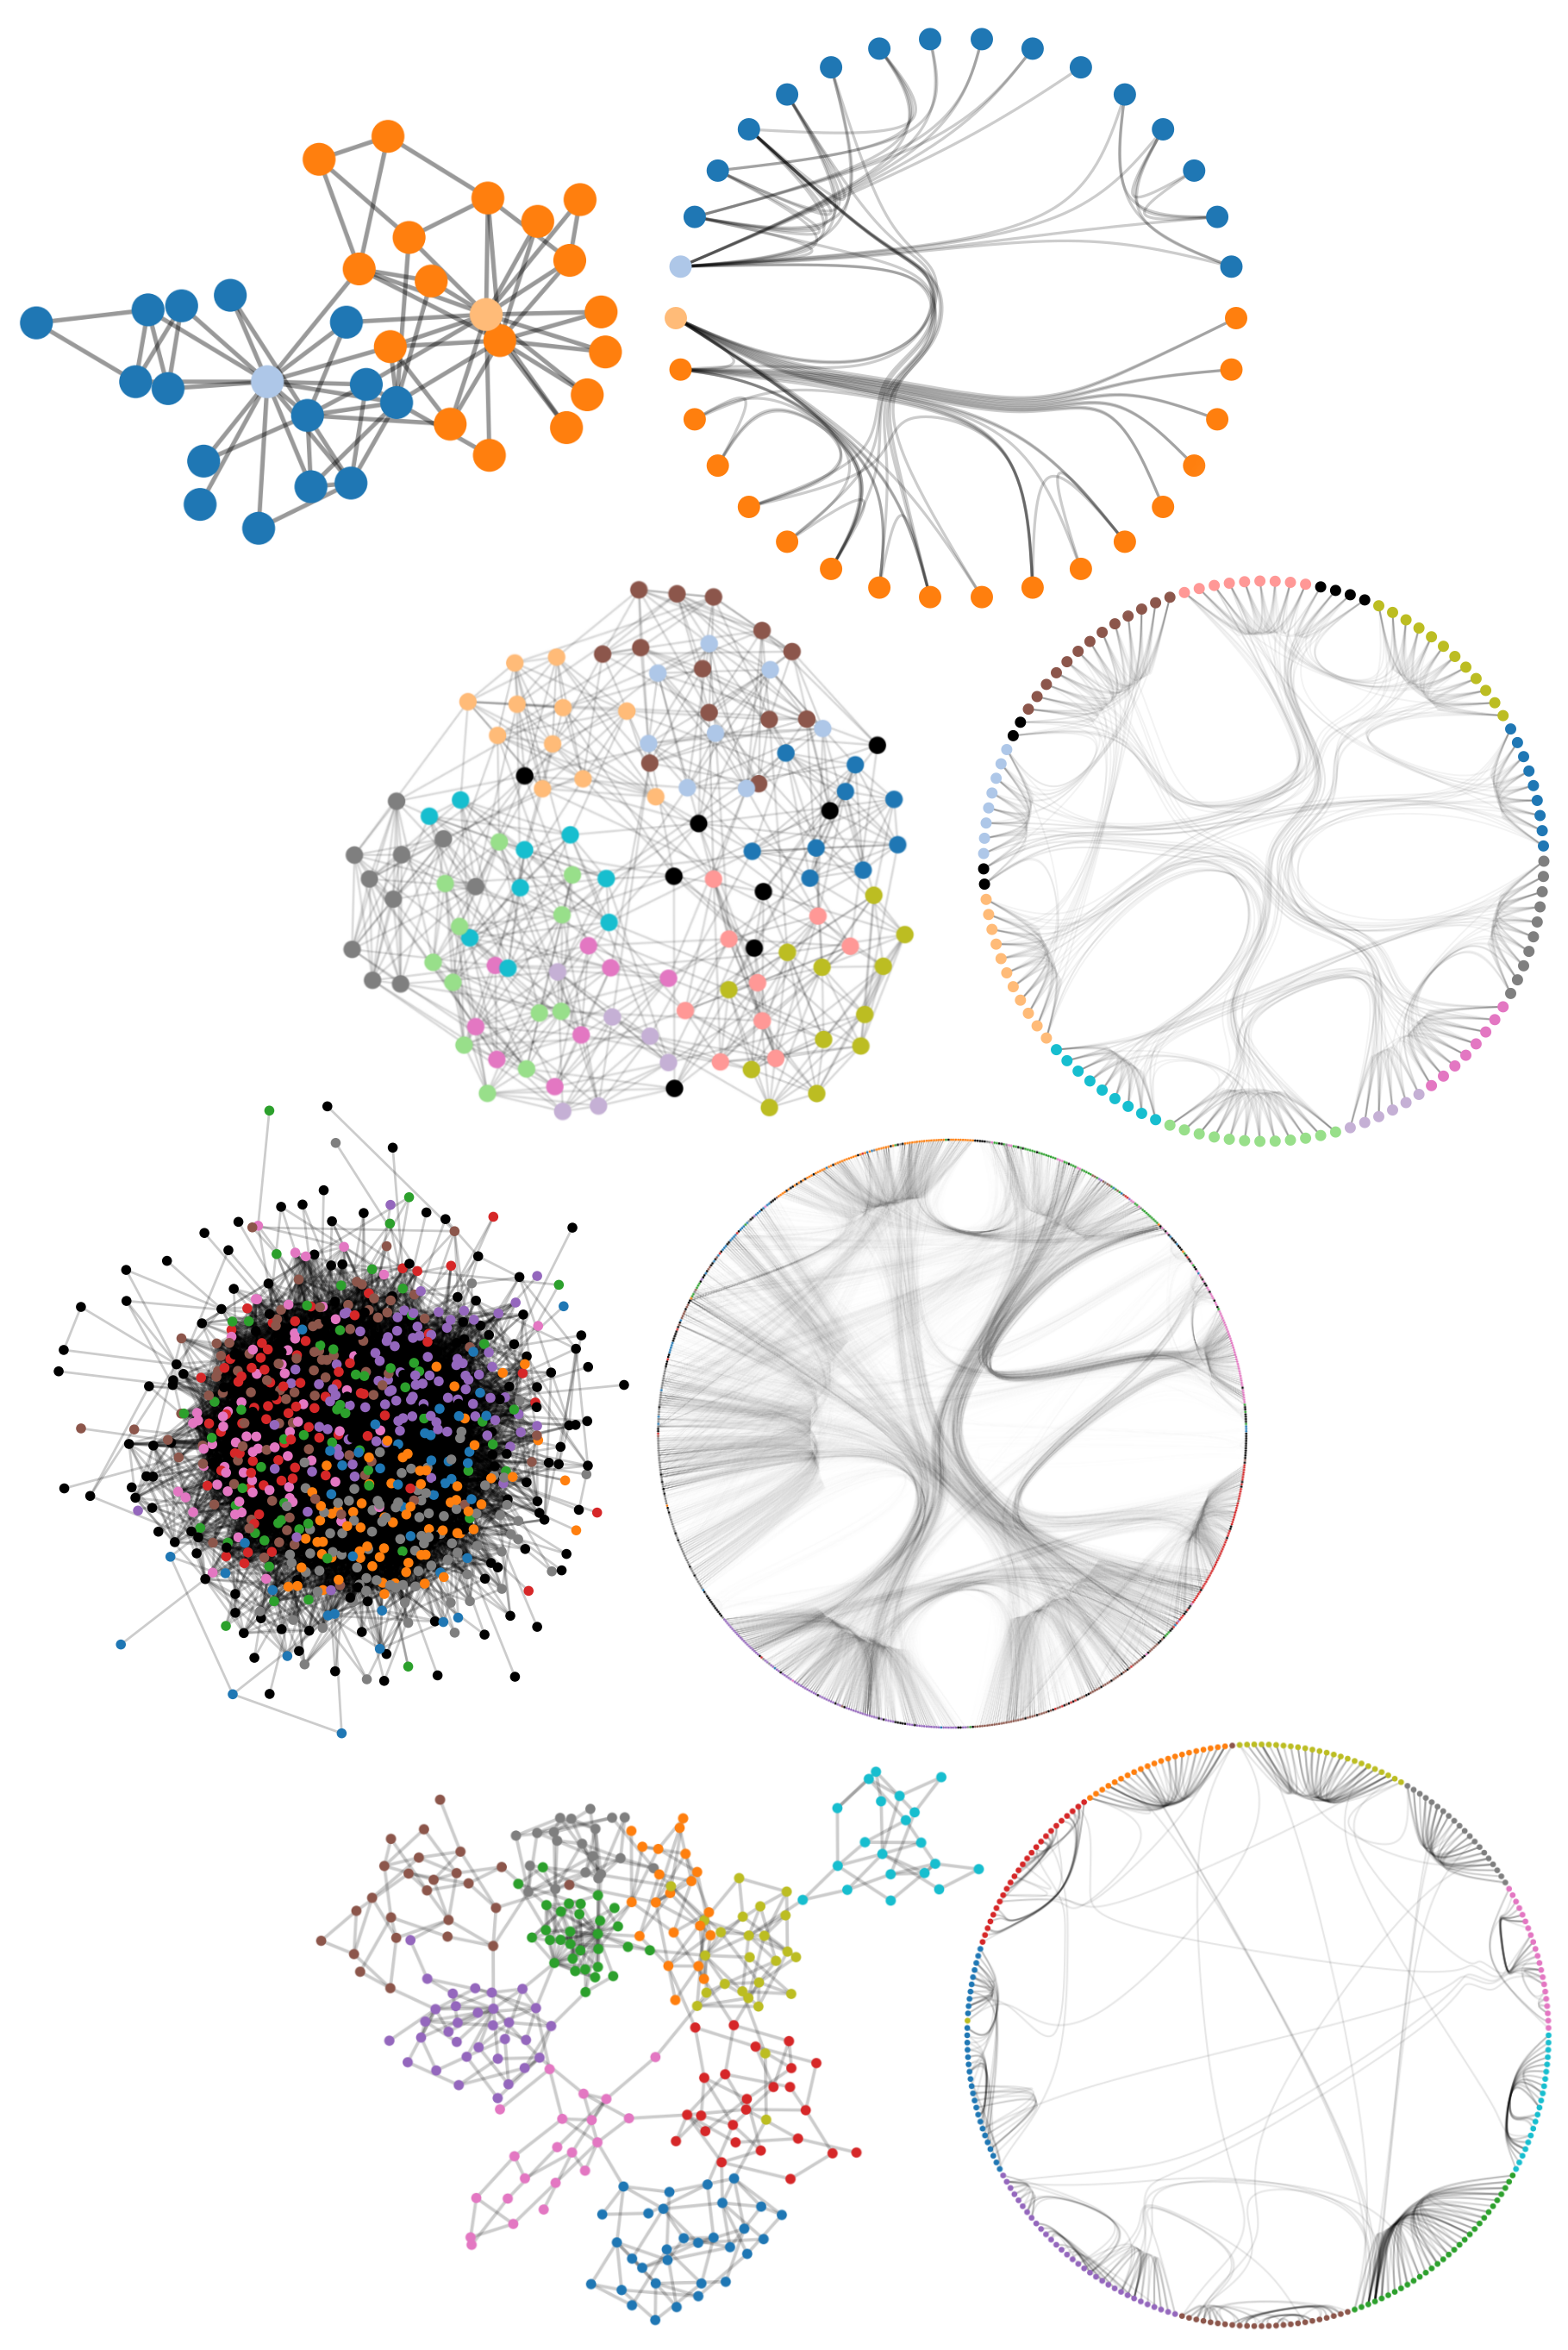
\includegraphics[height=.8\textheight]{power/bundled.png}
  \caption[Final hierarchical edge bundled diagrams]{Drawings of the graphs in Table~\ref{tab:bundle_graphs} using both a stress layout (left) and with hierarchical edge bundling (right). Colours of nodes correspond to the ground truth clusters included in the data. In \texttt{karate}, the two leaders of the club are coloured lighter.
  For \texttt{football}, 8 of its teams are singleton clusters in independent divisions, coloured black. For \texttt{caltech}, 168 students are unassigned to dorms, also coloured black.
  For all graphs, a branch merge distance of 10\% of the dendrogram height was used, with merged branches placed at a polar distance equal to the fraction of leaves it has as children, cubed.}
  \label{fig:untangled_hairballs}
\end{figure}


\subsection{Discussion}
\label{sec:heb_discussion}
The results presented here largely agree with the design choices made by Pons and Latapy \cite{Pons2006} for the use of agglomerative dissimilarity clustering on graphs. That is except for leaving out the extra $\mathbf{D}_{kk}^{\text{--}\sfrac{1}{2}}$ weighting in Equation~\ref{eq:walktrap} as it did not improve performance at all in the benchmark explored here.

The use of dissimilarity measures based on random walks outperforms those derived from other features such as shortest paths, as well as the GN algorithm used by Jia et al.\ \cite{Jia2011}, which also has a higher runtime complexity.
Calculating the betweenness-centrality for each edge is $\mathcal{O}(|V||E|)$ \cite{Brandes2001Centrality} and since this must be recalculated $|E|$ times, the overall complexity of GN is $\mathcal{O}(|V||E|^2)$, compared to $\mathcal{O}(|V|^2\log|V|)$ for the agglomerative methods explored here.
Ward's method also consistently outperforms other linkage methods, and a qualitative observation of note is that it also tends to give dendrograms that lend themselves more to the pruning process in Section~\ref{sec:pruning}. Branches in Ward dendrograms more clearly delineate separately groups of clusters, leading to easier simplification into a streamlined hierarchy for bundling.
% more systematic study into different methods for pruning 
When the opposite situation occurs, i.e.\ if differences in branch height are homogenous, the pruning process may merges every single branch into one, since child branches are recursively merged into their parents. However this also usually corresponds to a poor quality clustering in general, because the algorithm could not find large groups of datapoints all close to each other.
In a real-world visualisation pipeline, this pruning process would ideally be human driven, with methods such as MLCut of Vogogias et al.\ \cite{Vogogias2016} allowing dendrograms to be interactively explored and cut to form flat clusters. Such a tool could be easily applied to perform multiple cuts in order to form a hierarchy for bundling.
% trees can be interactively explored using \cite{Archambault2008}
Pruning is also not the only way to solve the dendrogram issues of Figure~\ref{fig:lesmis}. For example, different types of splines may not result in the same issues. A more thorough examination into the use of B-splines can be found in Section~\ref{sec:bspline_details}.

Interaction would also greatly improve the utility of these visualisations. Holten \cite{Holten2006} suggested ideas such as dynamically tweaking the amount that bundles are relaxed, and highlighting interesting bundles by hiding other links. An additional possibility in this context would be to interactively prune the hierarchical tree in order to neaten bundles, or being switching between different clustering algorithms to reveal different patterns depending on the algorithm selected.
The need for interaction can also be seen in the complex final render \texttt{caltech} in Figure~\ref{fig:untangled_hairballs}, second-from-bottom; an option such as \emph{GrouseFlocks} by Archambault et al.\ \cite{Archambault2008} would be useful here.

A quantitative assessment of the actual utility of resulting bundles is something missing from the literature, but out of scope for the work here.
It is however clear that certain topological features are made more salient by these diagrams. A good example of this is can be seen in the \texttt{karate} graph in Figure~\ref{fig:untangled_hairballs}, where it is clear that the two nodes on the left are central to the topology of the graph, due to the thickness of the bundles stemming from them. These two are in fact the two club leaders whose disagreement caused the club to split into the two factions used as ground truth for clustering. The algorithm was able to place them next to each other in a completely unsupervised manner, due to the quality of the extracted hierarchy combined with the optimal ordering \cite{Bar-Joseph2001} outlined in Section~\ref{sec:pruning}.
A possible study to quantify the effectiveness of bundles could be to ask participants to identify ground truth cliques or bicliques from different bundling configurations.

% Applying hierarchical edge bundles to the test set leads to smaller edges being within clusters and larger ones being across the 
Future work could also include testing on a larger benchmark, especially with graphs with more biclique than clique structure.
The current benchmark also measures the quality of clustering, but not bundling directly. A dissimilarity measure or energy function that quantifies bundling quality could be directly optimised to produce high-quality bundles.

% Another benefit to agglomerative methods is that it is easy to interpret and understand what the algorithm is doing, even if the answer is suboptimal. I would always pick an algorithm that I fully understand for a visualisation over a black-box algorithm that produces slightly better results. But this is just opinion.

\section{Power-confluent drawing}
\label{sec:power_confluent_drawing}
Edge bundling can be likened to data compression on graphs, as the goal is to describe a given network without having to know the source and target for every individual edge. 
Such compression would be impossible in a random network, but because real-world data does have structure, underlying patterns can be leveraged to group together similar components within the data.
% However, even knowing that this is the goal does not make the problem easier, because these underlying patterns are not known to us. The real world is complex, and so any data collected from it is not likely to be straightforward to understand. Much of the data collected may not even contain any order in the first place.
% In fact, if you will allow me to go meta for a moment, the very act of collecting data itself into the form of a network is already technically a form of compression, as 

The hierarchical edge bundling of the previous section can be interpreted as \emph{lossy} compression, because the bundling of edges can obscure the exact endpoints of each edge. In the same vein as, say, JPEG image compression, there exists a tradeoff between the amount of data used against the amount of information displayed.
But just as there exist lossless compression formats for images, such as PNG compression, there also exists a lossless counterpart for edge bundling, known as \emph{confluent drawing}. An example of such a drawing can be seen on the right-hand side of Figure~\ref{fig:power_teaser}, where the bundles are interpreted as follows: every possible smooth path from one vertex to another indicates that they are connected by an edge in the original graph.

This eliminates crossings by allowing edges to overlap, and is analogous to junctions on a train track that allow carriages to switch directions without stopping.

\begin{figure}
  \centering
  
\includegraphics[width=\textwidth]{power/teaser.pdf}
  \caption[A power-confluent drawing pipeline]{A pipeline for producing power-confluent drawings. 
  From left to right: a conventional node-link diagram with vertices arranged around a circle; its power graph decomposition, where edges are compressed by grouping similar verticess together; a novel equivalent routing graph, where the nested structure of groups is represented by a directed tree; the resulting confluent drawing, where original edges are threaded through the routing graph to form bundled junctions.}
  \label{fig:power_teaser}
\end{figure}

Confluent drawing has its roots in the more theoretical side of graph drawing, and was originally developed by Dickerson et al.\ \cite{Dickerson2005} as a novel method for drawing planar graphs. In Figure~\ref{fig:power_teaser} for example, the drawing of the original graph on the left contains many crossings and in fact can not be drawn in a planar way. Allowing edges to overlap, but requiring all smooth curves to denote an edge between endpoints, means that all connectivity is preserved, thus adhering to the analogy of lossless compression.
The precise definition of what defines a confluent drawing will be studied later in Section~\ref{sec:confluent_definition}.

The remaining work in this chapter will study a subset of confluent drawing known as \emph{power-confluent} drawing.
The process of producing a power-confluent drawing consists of three steps: finding the \emph{power graph decomposition;} converting this decomposition into an equivalent auxiliary routing graph (ARG), similarly to hierarchical edge bundling in Section~\ref{sec:pruning}; and finally drawing curves back on top to render a confluent drawing. Each step is illustrated in Figure~\ref{fig:power_teaser}. This was an idea originally explored by Bach et al.\ \cite{Bach2017}, and the work presented here will aim to further develop and formalise the methods there.
Specifically, the speed and quality of the first step will be improved, and two theoretical issues will be resolved for the second and third.

\subsection{Power graph decomposition}
\label{sec:power_graph}
A power graph is an extension to the conventional node-link diagram, that allows vertices to be grouped together into \emph{power groups}, in order to merge edges that share endpoints into individual \emph{power edges} (see the leftmost two drawings in Fig.~\ref{fig:power_teaser}). Power groups may also be nested in a hierarchical structure, allowing power edges to cross group boundaries.

This idea was originally developed for use in biological protein--protein interaction network analysis by Royer et al.\ \cite{Royer2008}, who originally computed a decomposition by using heuristics based on the Jaccard index, defined here in Equation~\ref{eq:jaccard}. This was later improved by Dwyer et al.\ \cite{Dwyer2014} who presented multiple methods of finding both optimal and sub-optimal decompositions, while also proving that the problem in general is likely to be $\mathcal{NP}$-hard. The method they recommended for practical use is a greedy agglomeration technique, not unlike the ones studied in Section~\ref{sec:dissimilarities}, except without the benefit of the Lance-Williams property shown in Equation~\eqref{eq:lancewilliams}. Its complexity is $\mathcal{O}(|V|^3|E|\log|E|)$, because it must search through $\mathcal{0}(|V|^2)$ merges $\mathcal{O}(|V|)$ times, and each merge takes $\mathcal{O}(|E|\log|E|)$ time to assess its quality. Here this assessment step will be improved slightly to $\mathcal{O}(|E|)$, and in practice the number of edges to be considered diminishes quickly anyway \cite{Dwyer2014}.

This is also the method chosen by Bach et al.\ \cite{Bach2017}, to construct their initial power graphs, and so is the one studied here. Note that the following description is specific to undirected graphs; the changes required for directed graphs are described in Section~\ref{sec:power_directed}.

\subsubsection{Greedy agglomeration, again}
The algorithm works taking advantage of the fact that the hierarchy of power groups can also be represented as a tree, with vertices as the leaves, similarly to the hierarchical clustering of Section~\ref{sec:dissimilarities}. It first initializes every vertex as the sole member of a trivial power group, henceforth referred to as a \emph{module}, and initializes a set of neighbours for each module based on the edges of the graph.
It then greedily merges pairs of top-level modules at a time, picking the merge that eliminates the most edges at each step, until no more edges can be eliminated.
The number of eliminated edges for any given merge is given by
\begin{equation}
  \kappa_{\cap}(m, n) = |N(m)\cap N(n)|
  \label{eq:kappa_cap}
\end{equation}
where $m$ and $n$ are modules and $N$ are their neighbour sets.
This is almost the same as $\mathrm{nedges}(m,n)$ in \cite{Dwyer2014}, except as a positive score rather than a negative penalty.
% See Dwyer et al. \cite{Dwyer2014} for detailed background and definitions.

This is the stage where the difference between this power decomposition and hierarchical clustering becomes clear: since power decomposition must preserve connectivity information, in line with the lossless compression analogy, care must be taken when performing the merging step in order to keep edges and power edges pointing at the correct endpoints. 
The simplest case is when two modules $m$ and $n$ share the exact same neighbours, i.e.\ $N(m)=N(n)$. In this case one module can simply be `absorbed' into the other, such that every pair of edges is merged into one, and the number of modules decreases by one. 

A trickier case is if only one of the modules contains edges that cannot be merged. For example, $m$ cannot fully absorb $n$ if $N(m)\supset N(n)$. Leaf modules of the hierarchical tree, i.e.\ individual vertices, also cannot be absorbed, and so the same situation occurs when $m$ is a leaf and $n$ is a module. In both cases $m$ adopts $n$, and $N(m)\cap N(n)$ is removed from $N(n)$.
If both contain edges that cannot be absorbed, i.e.\ $N(m)\not\subset N(n)$ and $N(m)\not\supset N(n)$, then a new module is created that adopts $m$ and $n$ as children and steals $N(m)\cap N(n)$ as its neighbour set. This also happens if $m$ and $n$ are both leaf modules.
Note that this is done equivalently in the original description by always generating a new parent module, and removing either child if their neighbour sets become empty \cite{Dwyer2014}.

However, measuring the reduction in edges as in Equation~\eqref{eq:kappa_cap} is not the only metric that a greedy algorithm can use to judge the quality of any given merge.
Only using one heuristic often results in many merges with the same score, and so the choice of merge may be arbitrarily chosen from many candidates, some of which may lead directly to local optima. In such situations it can be useful to include additional heuristics to further discriminate between choices.
This is not explicitly mentioned in \cite{Dwyer2014}, but is implemented in their provided source code, where they include two other metrics: minimising the total number of modules after the merge, and minimising the number of times power group boundaries are crossed by power edges.

Here a new heuristic will be introduced that can roughly capture the effects of both, and is simpler to calculate: a penalty for the number of edges that could not be merged. This is defined by
\begin{equation}
  \kappa_{\Triangle}(m, n) = |N(m)\,\Triangle\,N(n)|
  \label{eq:kappa_triangle}
\end{equation}
where $\Triangle$ denotes the symmetric difference, i.e.\ the number of unshared neighbours, between the two sets. This effectively measures the number of edges that cannot ever be eliminated in future steps, because only top level modules are considered for merging.
Equation~\eqref{eq:kappa_triangle} captures the number of modules because a new parent module is only added if both children have unshared neighbours, and so the smaller Equation~\eqref{eq:kappa_triangle} is, the fewer modules there will likely be. It also captures the effect of edges crossing group boundaries, because any unshared edges must cross the boundary of its new parent module after the merge.
Rewarding the first heuristic and punishing the second leaves a total score of
\begin{equation}
  \kappa(m,n) =
  w_\cap \kappa_\cap(m,n) -
  w_{\Triangle} \kappa_{\Triangle}(m,n)
  \label{eq:kappa_full}
\end{equation}
where $w_\cap$ and $w_{\Triangle}$ determine the relative weight of either heuristic. For example, to construct a modular decomposition \cite{Habib2004}, $w_{\Triangle}$ may be set to infinity to forbid any module boundary crossings.
Setting $w_\cap=10$ and $w_{\Triangle}=1$ works well in practice; these are the parameters used for the results in Table~\ref{tab:pgd_results}.

\begin{table}
  \centering
  \caption[Experimental results on greedy power graph decomposition]{Experimental results for the improved greedy power graph decomposition described in Section~\ref{sec:power_graph}
  $|E|$ is the number of edges in the original graph, compressed into $|P|$ power edges and $|M|$ power groups; shaded cells indicate the better score between the two methods.}
  
  \setlength{\tabcolsep}{1em}
  \renewcommand{\arraystretch}{1.25}
  \definecolor{grey}{RGB}{170,251,170} % mint :)

  \begin{tabular}{ |c|c|c|c|c| } 
    \hline
    \multirow{2}{*}{Name ($|E|$)} &
    \multicolumn{2}{c|}{Best $|P|$ $(|M|)$} & \multicolumn{2}{c|}{Worst $|P|$ $(|M|)$} \\ 
    \cline{2-5}
    & only $\kappa_\cap$ & $\kappa_\cap$ and $\kappa_{\Triangle}$ & only $\kappa_\cap$ & $\kappa_\cap$ and $\kappa_{\Triangle}$ \\ 
    \hline\hline
    \texttt{florentine} (20)
       % &\cellcolor{grey} 11 (4)
       % &\cellcolor{grey} 11 (4)
       & 11 (4)
       & 11 (4)
       & 11 (6)
       &\cellcolor{grey} 11 (5) \\
    \texttt{karate} (78)
       % &\cellcolor{grey} 28 (13)\
       % &\cellcolor{grey} 28 (13)
       & 28 (13)\
       & 28 (13)
       & 30 (15)
       &\cellcolor{grey} 29 (13)\\ 
    \texttt{southern} (89)
       & 30 (17)
       &\cellcolor{grey} 27 (21)
       & 37 (16)
       &\cellcolor{grey} 30 (18)\\ 
    \texttt{dolphins} (159)
       & 82 (29)
       &\cellcolor{grey} 81 (30)
       & 87 (28)
       &\cellcolor{grey} 83 (30)\\ 
    \texttt{lesmis} (254)
       & 74 (39)
       &\cellcolor{grey} 72 (41)
       & 79 (39)
       &\cellcolor{grey} 72 (42)\\
    \texttt{football} (613)
       & 282 (83)
       &\cellcolor{grey} 278 (84)
       & 289 (83)
       &\cellcolor{grey} 286 (84)\\
    \texttt{netsci} (914)
       & 355 (187)
       &\cellcolor{grey} 338 (184)
       & 371 (189)
       &\cellcolor{grey} 341 (186)\\
       
    \hline
  \end{tabular}
  \label{tab:pgd_results}
\end{table}

Adding the new heuristic produces the best or joint best results in all graphs, and also improves the consistency of the output, with a better worst result in all cases.
% The improvements are small, but are consistently better and with less variance.
Note that the variation between runs in the implementation used is due to a pseudorandom order of iteration through
candidate merges (Figure.~\ref{fig:pseudo_pgd}, line~\ref{code:pgd:top}).
% \texttt{std::unordered\_set} in \Cpp, which may vary between implementations of the standard library.
The networks are, from top to bottom, Italian families linked by marriage \cite{Breiger1986}, members of a karate club \cite{Zachary1977}, women meeting at social events \cite{Davis2009}, interactions between bottlenose dolphins \cite{Lusseau2003}, co-occurrence of characters in the musical Les Mis\'erables \cite{Knuth1993}, American football games between US colleges \cite{Girvan2002}, and coauthorships of scientists working on network theory \cite{Newman2006Eigenvectors}.
 
\begin{figure}
  \removeAlgorithmFigureError
  \DontPrintSemicolon
  \begin{algorithm}[H]
    \SetKwInOut{Input}{inputs}
    \SetKwInOut{Output}{output}
    \SetKwFor{ForEach}{foreach}{}{}
    \SetKwRepeat{Do}{do}{while}
    \SetKwIF{If}{ElseIf}{Else}{if}{}{else if}{else}{}
    \Input{graph $G=(V,E)$}
    \Output{modules $M=\text{set of pairs }(C,N)$}
    
    $M \leftarrow \{(\emptyset,\,N(v))\ |\ v\in V\}$
    
    \Do{$\kappa_\mathrm{best}>0$}{
      $\kappa_\mathrm{best}\leftarrow0$
      
      \ForEach{\emph{pair of modules} $\{m,n\}\in M_\mathrm{top}\times M_\mathrm{top}$}
      {
        \label{code:pgd:top}
        $\kappa_\mathrm{best} \leftarrow \max(\kappa(m,n),\,\kappa_\mathrm{best})$
        \label{code:pgd:kappa}
      }
      $\textsc{merge}(\{m,n\}_\mathrm{best})$
      \label{code:pgd:merge}
    }
    \caption{\textsc{Greedy power graph decomposition}}
    \label{alg:pgd}
  \end{algorithm}
  
  \caption[Pseudocode for improved power graph decomposition]{Pseudocode for the greedy heuristic power graph construction in Section~\ref{sec:power_graph}.
  Each module consists of a set of children $C$, and a set of neighbours $N$.
  The score function $\kappa$ is from Equation~\eqref{eq:kappa_full}, and the merge operation on line~\ref{code:pgd:merge} is described in Section~\ref{sec:power_graph}, where any new module is parented to its merged children by adding them to its set of children $C$.
  In practice a redundant super-module is maintained, whose children are the top level modules $M_\mathrm{top}$ on line~\ref{code:pgd:top}.}
  \label{fig:pseudo_pgd}
\end{figure} 

It is important to note that this is still a simple greedy heuristic, which does not make any guarantees about the quality of the final result.
The original method in \cite{Dwyer2014} gives the option to somewhat alleviate this, by optionally maintaining a priority queue of the best configurations seen so far, along with some dynamic programming to prevent re-evaluating configurations already seen.
A further exploration of this extended algorithm is out of scope for this paper, and Dwyer et al. \cite{Dwyer2014} additionally note that the qualitative improvement that results from including this priority queue is minimal.

The final change involves bringing down the complexity of neighbour set intersection to $O(E)$ using hash sets, which reduces the complexity of the algorithm down slightly to $O(|V|^3|E|)$.
Pseudocode for the above described algorithm can be seen in Fig.~\ref{fig:pseudo_pgd}.

\subsection{Confluent drawing}
\label{sec:confluent_definition}
The original definition of a confluent drawing~$A$ for a graph~$G$ is:
\begin{mdframed}[backgroundcolor=WhiteSmoke]
\begin{itemize}[leftmargin=*]
  \item There is a one-to-one mapping between the vertices in $G$ and $A$, so that, for each vertex $v\in V(G)$, there is a corresponding vertex $v'\in A$, which has a unique point placement in the plane.
  % \item There is an edge $(v_i,v_j)$ in $E(G)$ if and only if there is a locally-monotone curve $e'$ connecting $v_i'$ and $v_j'$ in A.
  \item There is an edge $(v_i,v_j) \in E(G)$ iff there is a locally-monotone curve [defined as having no self intersections or sharp turns] $e'$, connecting $v_i'$ and $v_j'$ in $A$. 
  \item $A$ is planar. That is, while locally-monotone curves in $A$ can share overlapping portions, no two can cross.
\end{itemize}
\end{mdframed}
This was proposed by Dickerson et al.\ \cite{Dickerson2005}, where the second condition is the key part of the definition that lets links overlap in the final drawing.
It is not immediately obvious how to convert a power graph into such a drawing. Fortunately, Bach et al.\ \cite{Bach2017} proposed the idea of first converting a power graph decomposition into an ARG. Then, for each adjacency, the graph-theoretic shortest path through the ARG is used as the sequence of control points for a B-spline \cite{Sederberg2005}.

This process is illustrated in Fig.~\ref{fig:power_teaser}, and the ARG used is almost exactly the one in hierarchical clustering (Section~\ref{sec:heb_background}), where each layer of the hierarchy is mapped to a branch vertex in a hierarchical tree.
The only differences are the removal of the root of the tree, and the addition of extra edges between tree vertices to represent power edges, as shown in Figure~\ref{fig:power_teaser}, second from right. Note that the in the original algorithm \cite{Bach2017} edges in the ARG are undirected, unlike those shown in Figure~\ref{fig:power_teaser}.
The addition of directed edges to the ARG will be used to solve the theoretical issues outlined below, in Section~\ref{sec:hierarchical_routing}.

It will be shown here that the original combination of B-splines and shortest paths introduces problems not fully explored by the original authors, causing the resulting drawings to violate the second and third conditions in the above definition. These problems will be solved, and the subclass of confluent drawings the algorithm can produce will be identified as a new classification known as \emph{power-confluent}. The fixed solution guarantees that the second condition is always satisfied, but still cannot guarantee the third, as discussed in Section~\ref{sec:power_planarity}.

\subsubsection{Problem 1: Node splitting}
\label{sec:node_split}
Issues regarding the use of B-splines are first identified (of degree $p=3$ in the source code of \cite{Bach2017}, although it is not specified in the paper) for interpolating control points.
These were likely chosen because they satisfy the convex hull property, which prevents crossings at shared control points. They also offer local control (i.e.\ moving a control point only affects the surrounding $p+1$ segments), which guarantees that splines that share enough intermediate control points will overlap.
Local control is what makes it possible for drawings to be confluent; with the right routing graph, it is possible for edges to share enough control points to produce the overlapping portions that are required for a confluent drawing. Specifically, for two curves to be guaranteed to overlap they must share $p$ or more control points (see Section~\ref{sec:bspline_details} for a proof and a more detailed explanation).

\begin{figure}
  \centering
  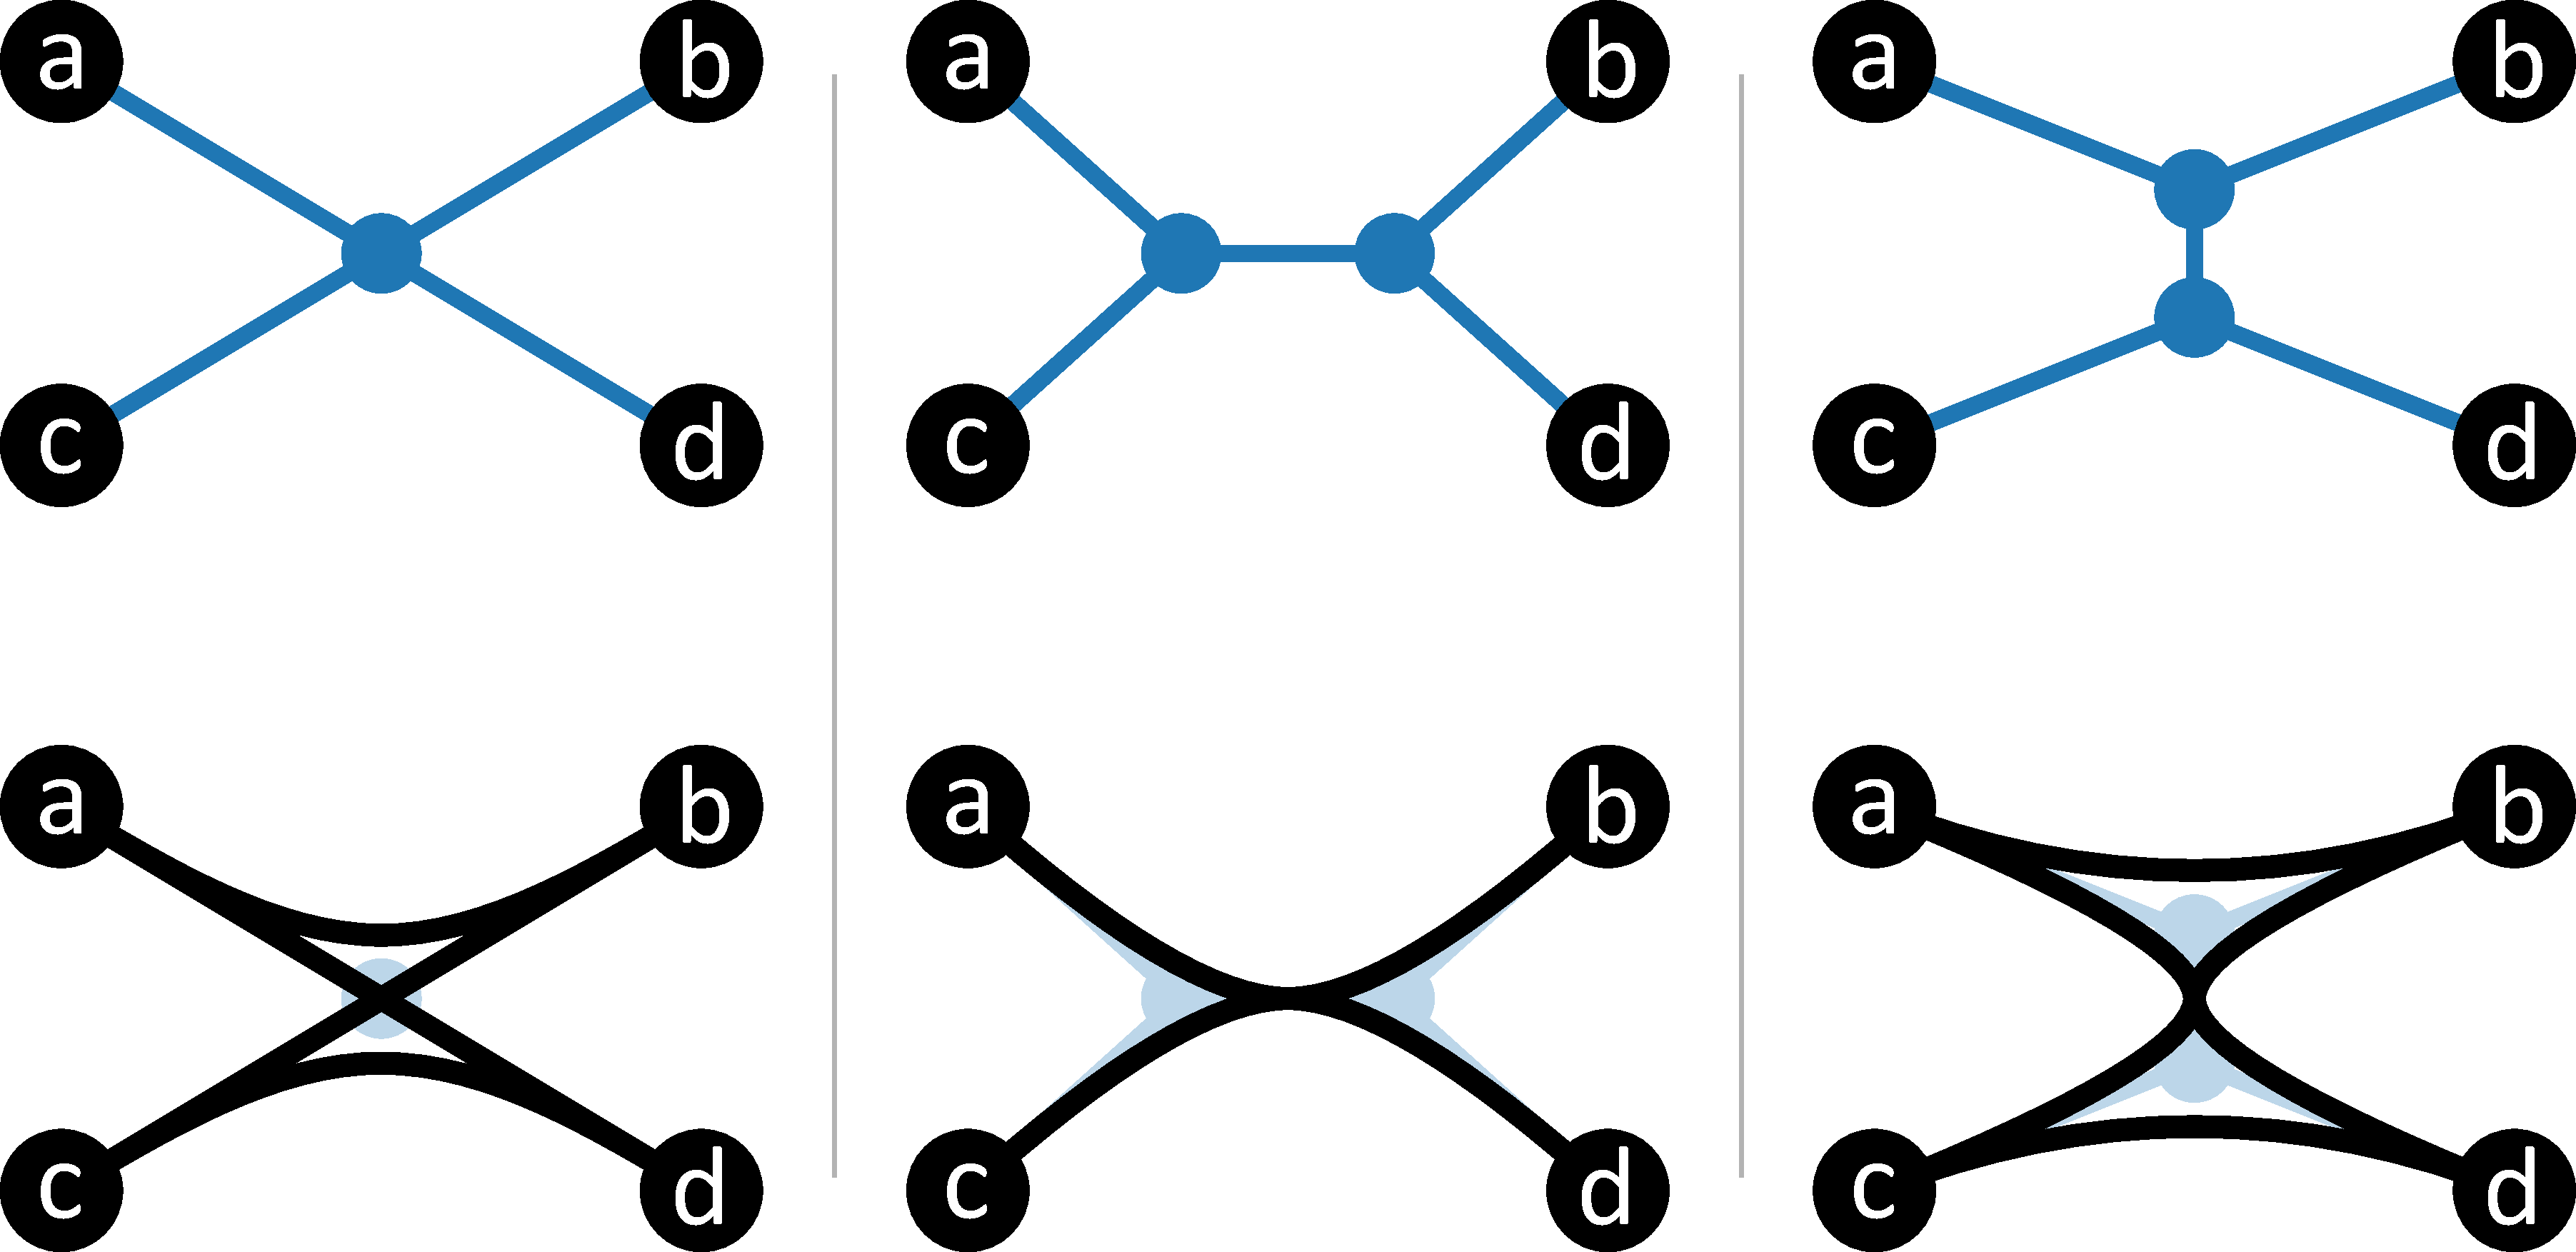
\includegraphics[width=.8\textwidth]{power/nodesplit.pdf}
  \caption[Examples of the node split problem]{Examples to show how the direction of node splitting can affect the graph $K_{2,2}$. The first column shows a standard situation where a split is required to make edges overlap, the second shows the correct split, and the third shows that if the node is split the other way, then the edges $\{a,c\}$ and $\{b,d\}$ are falsely introduced.
  }
  \label{fig:nodesplit}
\end{figure}

There are two problems with using B-splines in this context. The first is that splines that share fewer than $p$ control points will \emph{not} overlap, but sharing even a single routing node should indicate a bundled junction.
The authors recognized this, calling it the `crossing artifact' \cite[Fig.~4]{Bach2017}, and fixed it by splitting routing nodes into two: one for incoming and one for outgoing edges.
The intuition behind this splitting is correct, as it introduces another shared control point that tightens the bundle, joining the crossed edges into a junction. However, their exact description contains an ambiguity in the context of undirected graphs, as it is not specified how to identify edges as incoming or outgoing. This is problematic as an incorrect split may introduce errors into the resulting drawing, as illustrated in Figure~\ref{fig:nodesplit}.
This ambiguity will be resolved, along with the following related problem, in Section~\ref{sec:hierarchical_routing}.

The second problem is also caused by local control but has an opposite result: that splines will \emph{always} overlap if they share $p$ or more control points.
For some ARGs, such as the examples in Figure~\ref{fig:overlap}, splines may overlap so as to create the visual impression that extra edges, not present in the original graph, exist. This violates the second condition in the confluent definition.
Such an ARG can result from the power-to-routing graph conversion, as explained in the following section.

\subsubsection{Problem 2: Short-circuits}
\label{sec:short_circuits}
Here it will be explained why routing edges through their graph-theoretic shortest paths in the ARG can introduce false adjacencies.
% A power graph is an extension to the conventional node-link diagram, that compresses the number of edges by grouping similar vertices together into \emph{power groups}, and merging edges among group members that share the same target vertex into a single \emph{power edge} instead (see the leftmost two drawings in Figure~\ref{fig:power_teaser}).
A power decomposition is converted into an ARG by (a) connecting the members of each power group to a new vertex corresponding to the group, and (b) connecting pairs of vertices whose corresponding power groups are connected by power edges.
% The hierarchical structure of power decompositions means that (a) forms a tree, and (b) forms bridges between vertices in that tree.
\begin{figure}
  \centering
  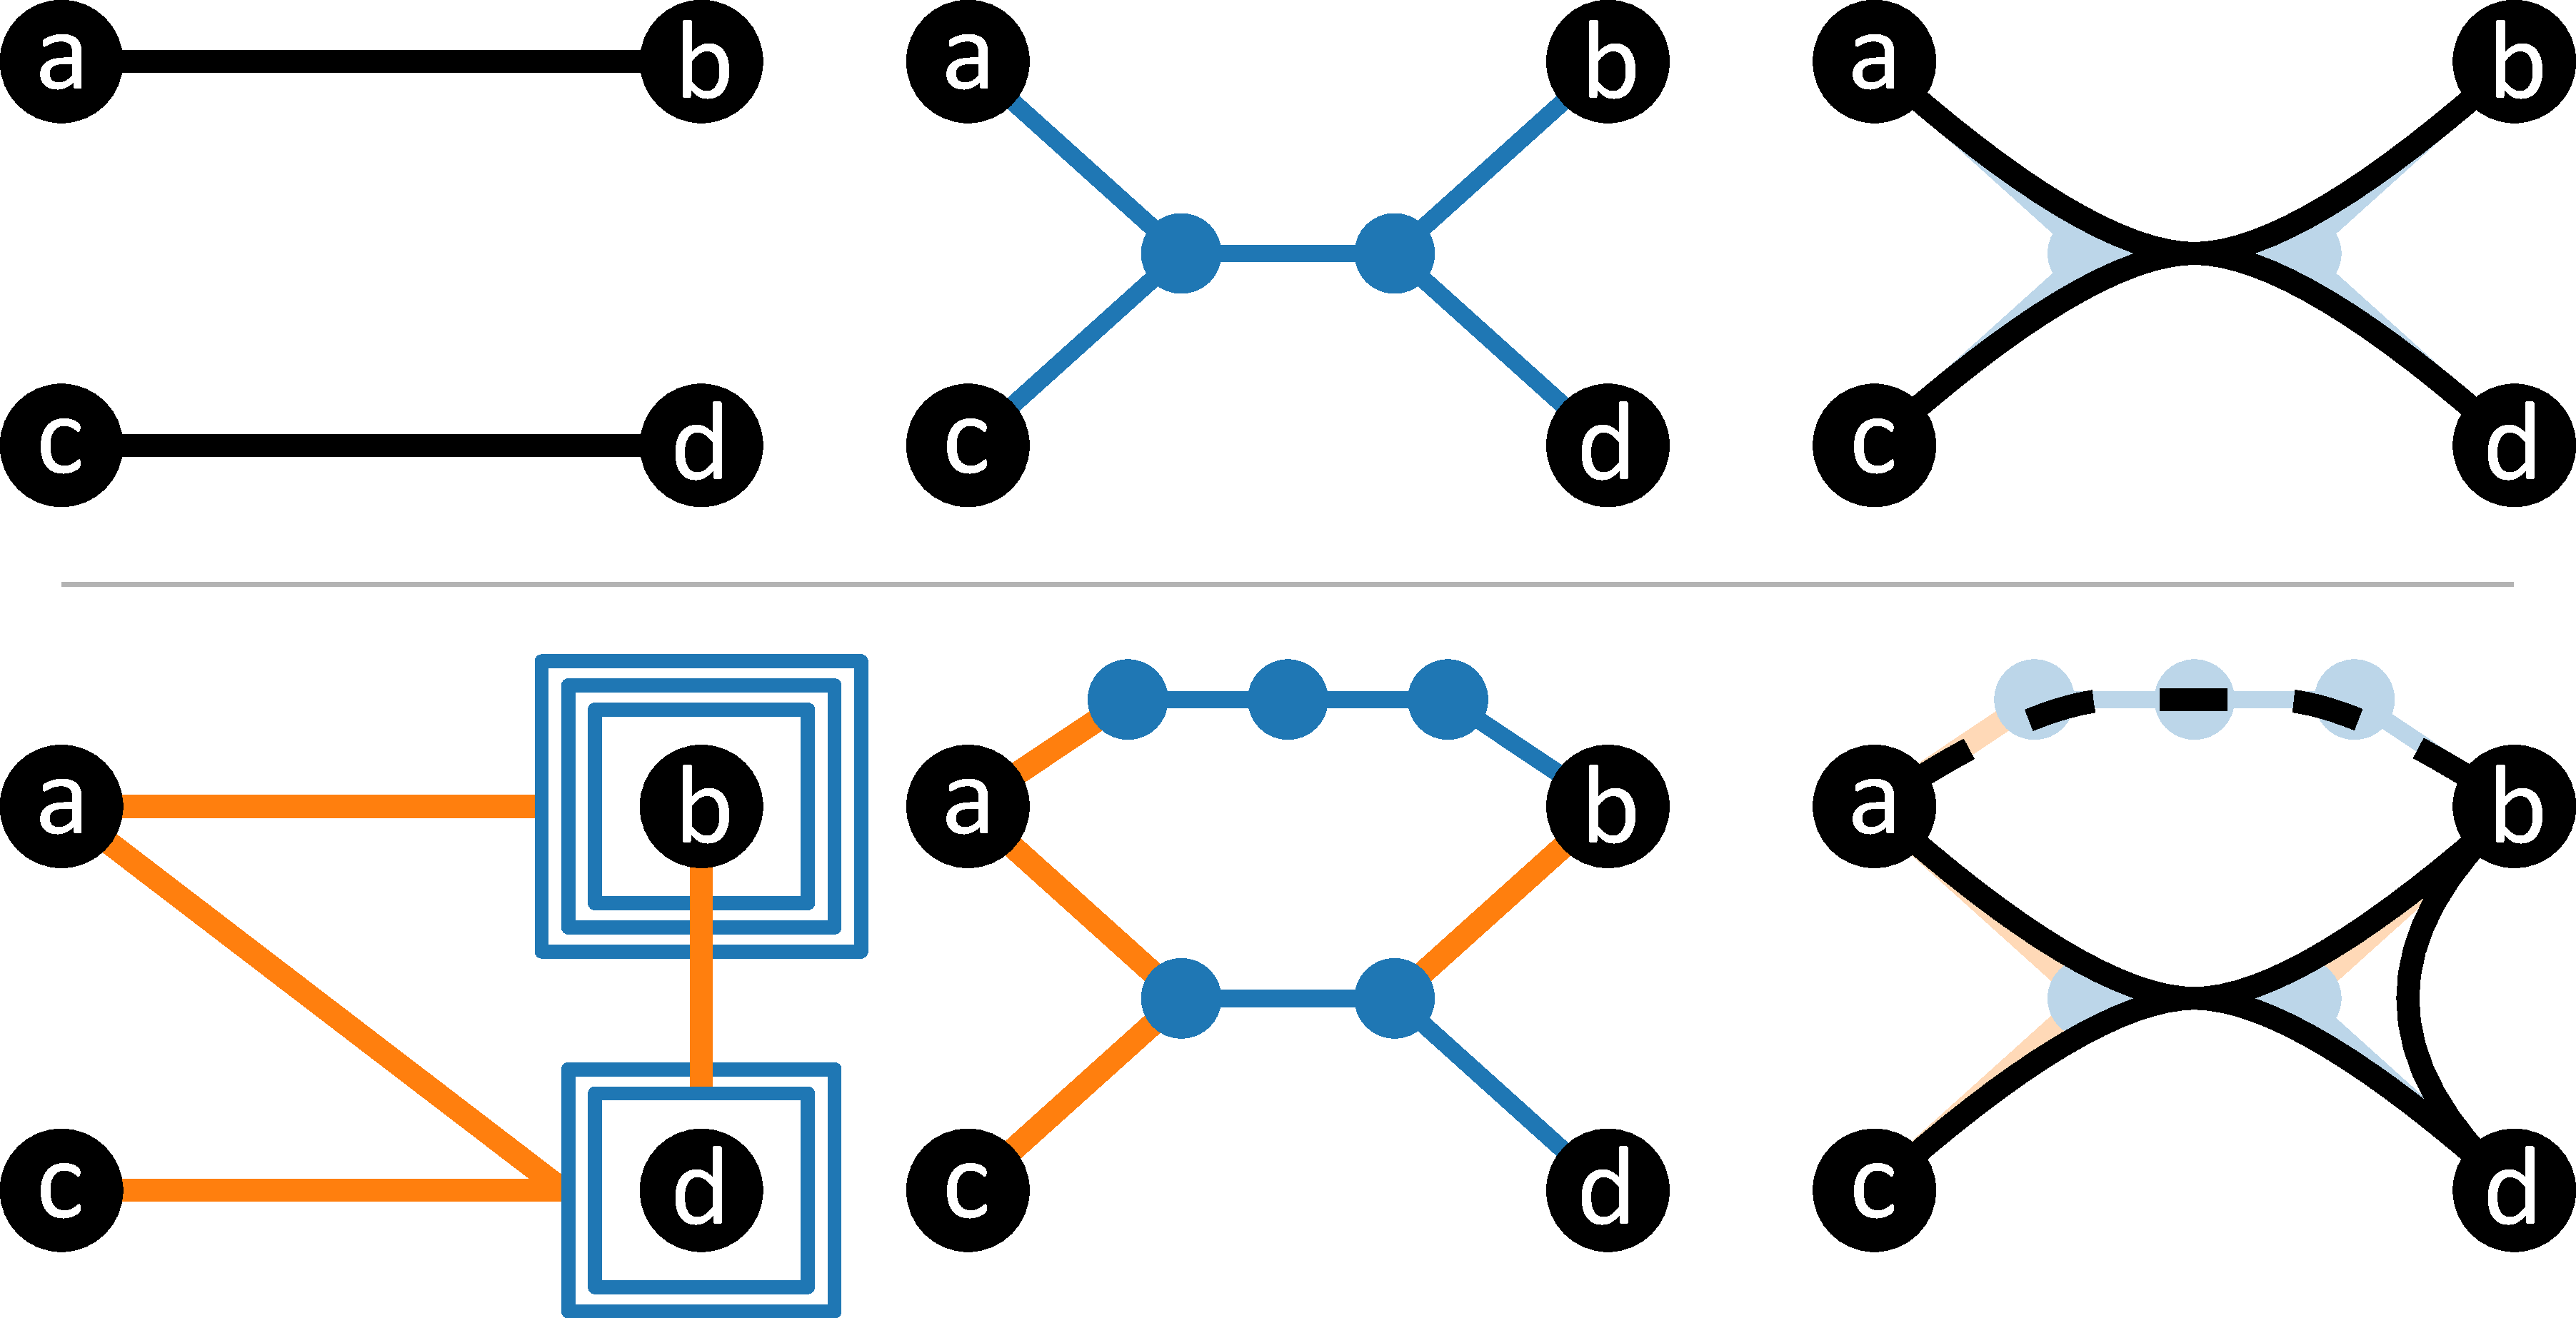
\includegraphics[width=.8\linewidth]{power/shortcircuit.pdf}
  \caption[Examples of the short-circuit problem]{Examples of how absent edges can appear to exist due to the short-circuit problem.
  Top: a toy example of a hypothetical routing graph that causes edges $\{a,d\}$ and $\{c,b\}$ to both erroneously appear to exist.
  Bottom: an example of a power graph that causes a similar ambiguity, where $c$ appears connected to $b$ because the edge $\{b,d\}$ short-circuits the nested structure of power groups (represented by blue boxes), causing $\{a,b\}$ to be routed incorrectly downwards.
  The correct direction that would not cause an issue is shown as a dashed line along the top.
  }
  \label{fig:overlap}
\end{figure}
\begin{figure}
  \centering
  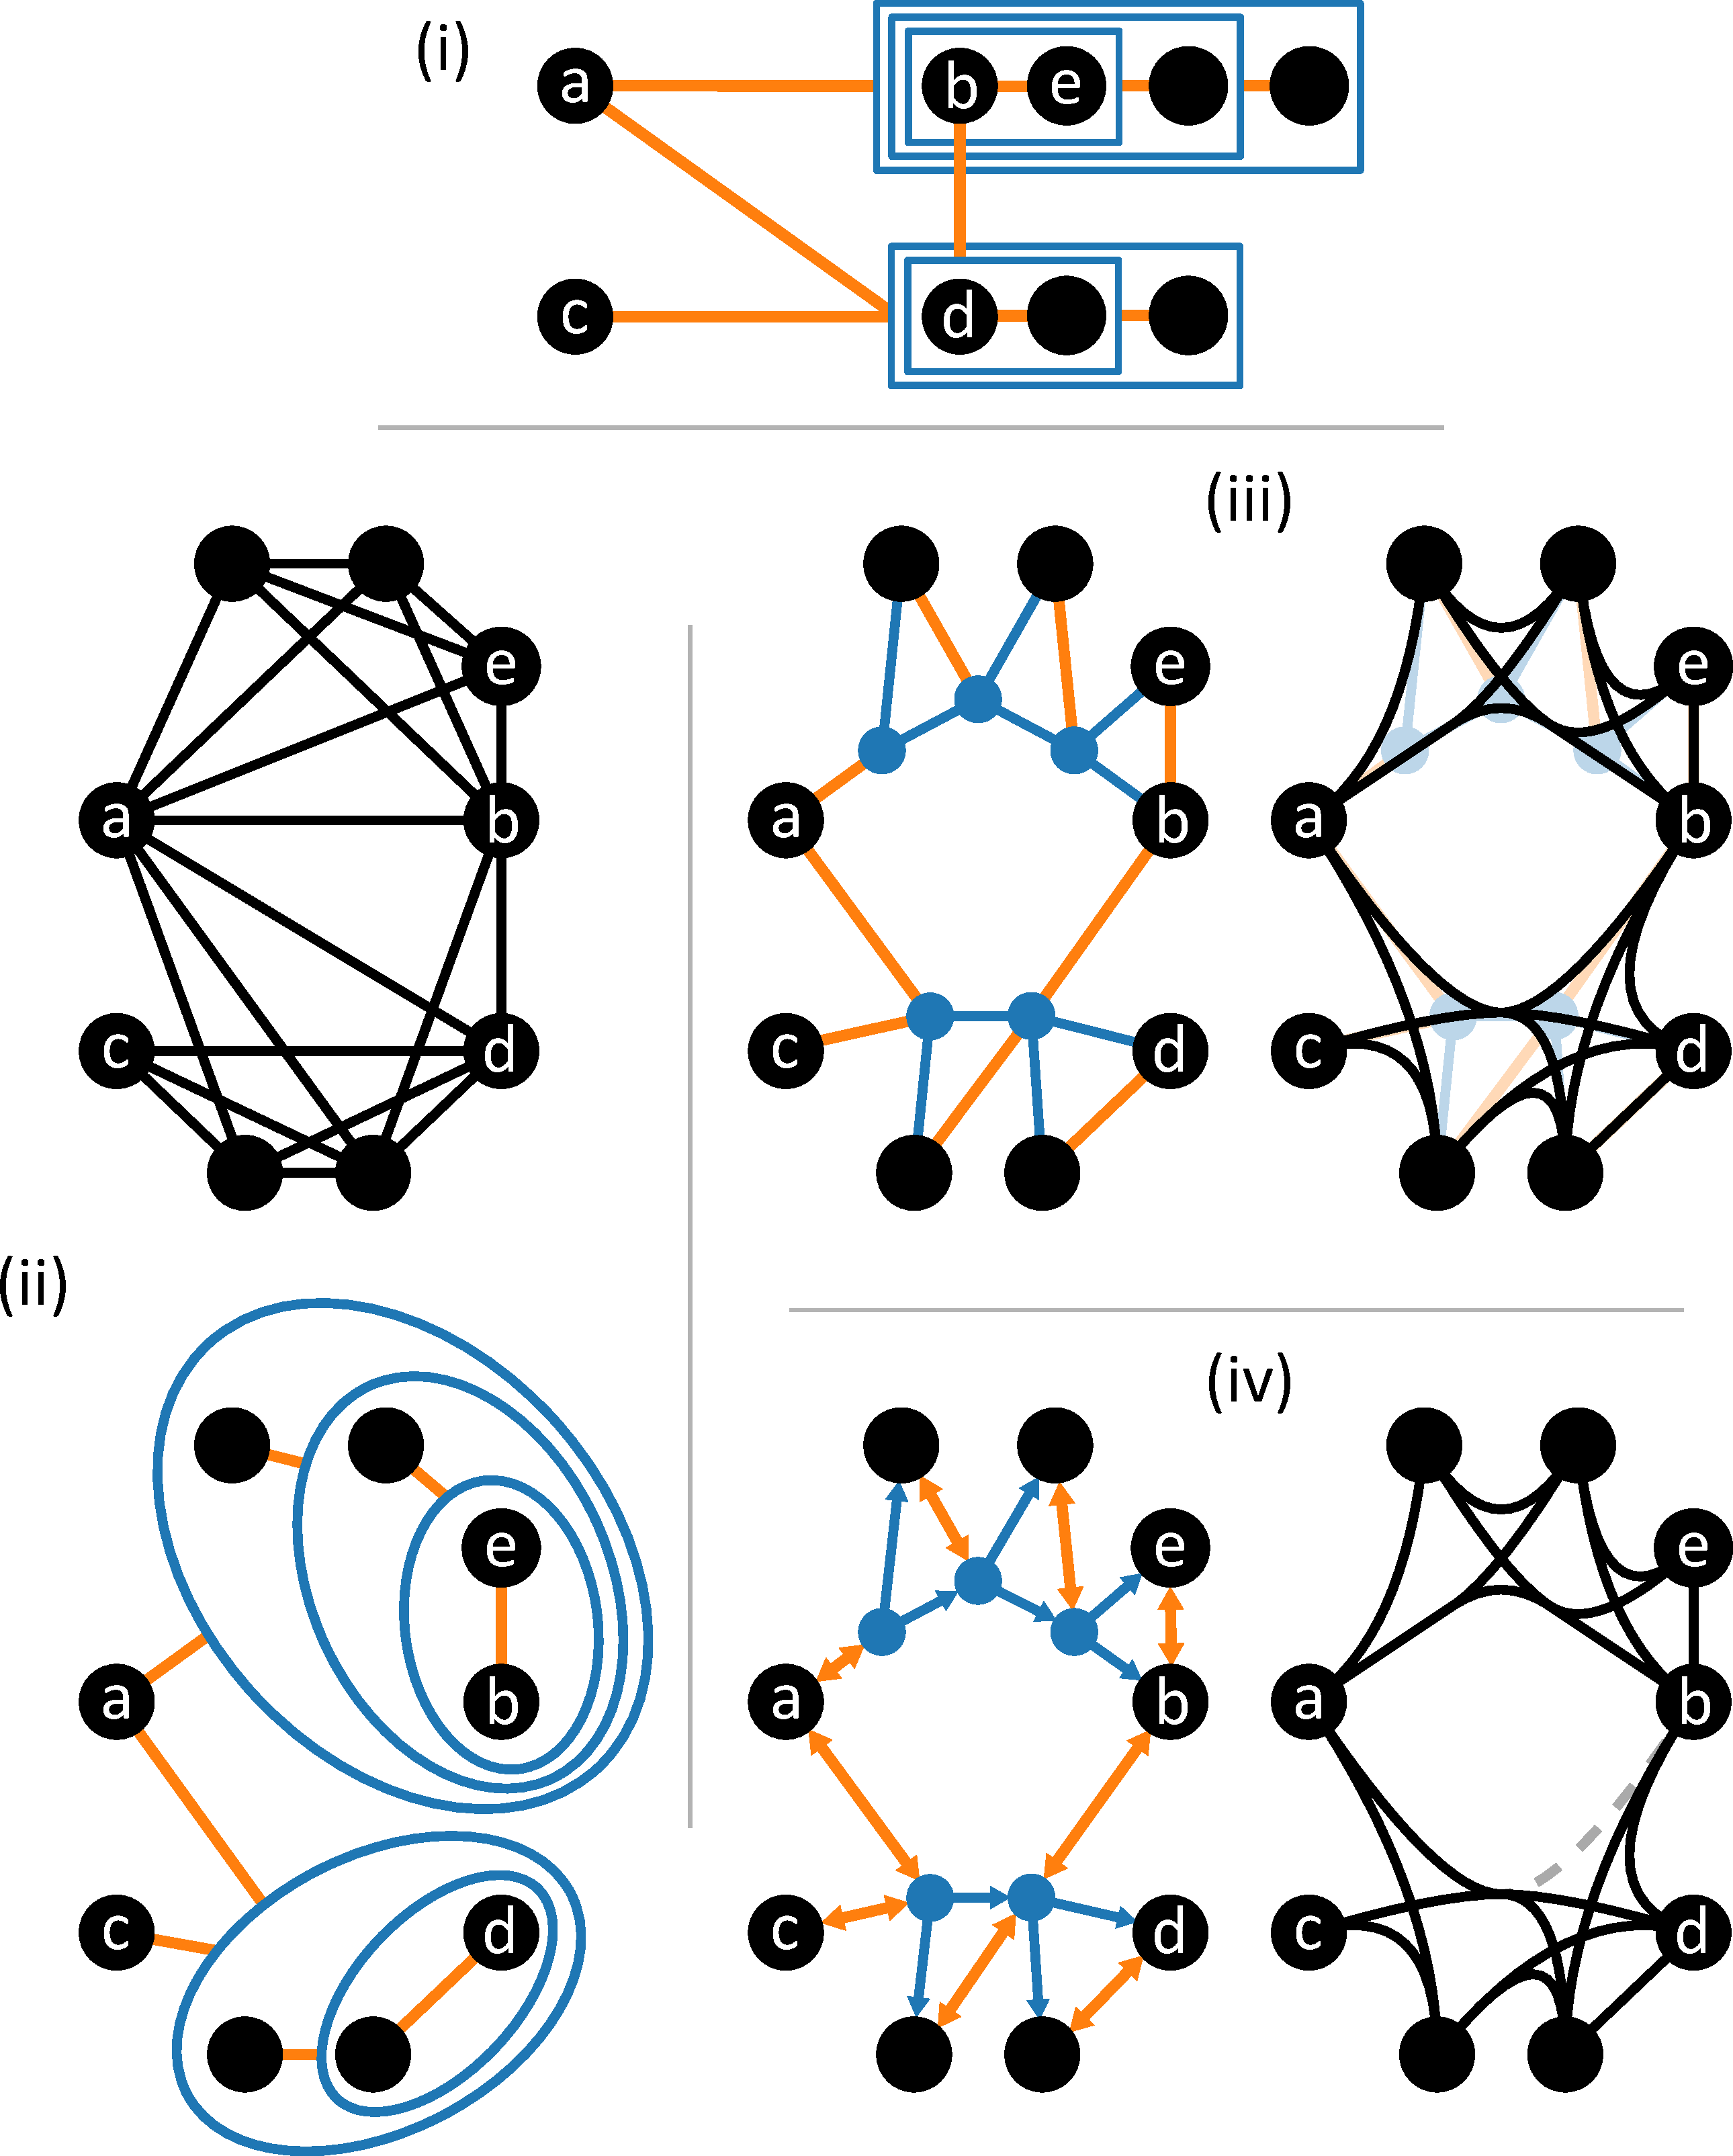
\includegraphics[width=.8\linewidth]{power/shortcircuit_big.pdf}
  \caption[A full version of Figure~\ref{fig:overlap}]{A fleshed-out version of Figure~\ref{fig:overlap}, bottom, without any redundant power groups.
  (i): an example of the power graph in the same layout as Figure~\ref{fig:overlap}, where the nested structure of groups comes from a clique structure.
  (ii) top: a conventional node-link layout of the graph, bottom: the same power graph as in (i). 
  (iii) left: the resulting routing graph from the method of Bach et al.\ \cite{Bach2017}, right: the resulting drawing when splines take their shortest paths through this routing graph. The edge $\{a,b\}$ is routed downwards in the wrong direction, causing the edge $\{c,b\}$ to falsely appear to exist.
  The edge $\{a,e\}$ also has two equal-length shortest paths, either through the line shown or downwards through $b$.
  % , albeit this specific case can easily be prevented by only preventing original nodes from being used as intermediate control points, as the original authors appear to have done in \cite[Fig.~2(c)]{Bach2017} for the edge $\{u,w\}$.
  (iv) left: the result of using the new method (Section~\ref{sec:hierarchical_routing}) of retaining the hierarchical structure of power groups through directed edges, right: the resulting drawing where $\{a,b\}$ is routed through the three correct upward routing nodes. The previously incorrect routing is marked by a dashed line.
  }
  \label{fig:overlap_sm}
\end{figure}
Since the original edges do not exist in this auxiliary graph, they are instead drawn back on top by finding the graph-theoretic shortest path between the vertices on either end of the edge, using the nodes on this path as the control points for a spline.
However, since (a) and (b) both result in edges in the routing graph, with nothing to differentiate between them, this can cause a \emph{short-circuit} effect, that potentially introduces false adjacencies into the resulting drawing.
This is shown in Figure~\ref{fig:overlap}, where two intermediate routing nodes are used because that is the minimum number of shared control points required for quadratic splines to overlap (see Section~\ref{sec:bspline_details}).
Note that every power group in this example is intentionally redundant for clarity; a full version of this example can be seen in Figure~\ref{fig:overlap_sm}.

This effect can be explained as follows. The structure of groups within a power graph can be represented as a tree, where groups are represented by branches and vertices by leaves.
Trees are geodetic (i.e.\ there exists a unique shortest path between any pair of vertices), but the connections introduced by power edges can act like bridges between branches, to invalidate this property and produce ambiguity either in the choice of path (if the shortest paths are equal) or in which edges exist at all, by routing splines in the wrong direction entirely.
% This violates the second condition in the definition of confluent.
% In any case it does not matter how often the corner case appears; if it exists then the method cannot be defined as confluent.
The bottom row in Figure~\ref{fig:overlap} shows a simple example of how this can happen. While it may seem as if this counter-example is contrived and should not ever appear due to the redundant nested structure of power groups, a similar pattern arises from the optimal decomposition of a clique, shown in Figure~\ref{fig:overlap_sm}.
The key detail here is that only one power edge should ever be traversed for any given adjacency, which is guaranteed by the solution described in the following Section~\ref{sec:hierarchical_routing}.

\subsection{Hierarchical routing}
\label{sec:hierarchical_routing}

% The solution to these problems is to retain the hierarchical structure of power groups as a directed tree, with all routing edges directed towards the leaves. Power edges are then added back, except as a special type of edge that is incoming at both ends (the purpose of which will soon be made clear). If the root of the tree is then discarded, what is left is the exact same ARG as before, except now with all routing edges explicitly directed (see Figure~\ref{fig:radial}, middle column).
The solution to these problems is to instead construct the ARG as follows:
\begin{mdframed}[backgroundcolor=WhiteSmoke]
\begin{itemize}[leftmargin=*]
  \item The hierarchical structure of power groups is retained as a directed tree, with all routing edges directed towards its leaves.
  \item Power edges are reattached between their corresponding branch vertices, as a special type of routing edge that is incoming at both branch vertices.
  \item The root of the tree is discarded.
\end{itemize}
\end{mdframed}
This leaves the same ARG as before, except now with all routing edges explicitly directed (see Figure~\ref{fig:radial}, middle column).
Note that this also means all adjacency information is now preserved in the ARG, such that the original graph can be recovered.
The purpose of having power edges outgoing at both ends will soon be made clear.


\begin{figure}
  \centering
  \includegraphics[width=.8\linewidth]{power/solution.pdf}
  \caption[A fixed method for confluent drawing]{The solution to both ambiguities described in Section~\ref{sec:hierarchical_routing}.
  % The same example graph as in \cite[Fig.~2]{Bach2017} and here Figure~\ref{fig:power_teaser} is used, shown in a radial layout to emphasize the tree structure of power groups.
  The leftmost graphs are a power graph (top), and a tree that represents the hierarchy of power groups (bottom), but without power edges.
  The middle column contains the resulting routing graphs without node splitting (top) and with (bottom, split indicated in red).
  % Note that these do not include or require the root of the tree.
  The final column displays the resulting bundled layouts.
  }
  \label{fig:radial}
\end{figure}

\begin{figure}
  \removeAlgorithmFigureError
  \DontPrintSemicolon
  \begin{algorithm}[H]
    \SetKwInOut{Input}{inputs}
    \SetKwInOut{Output}{output}
    \SetKwFor{ForEach}{foreach}{}{}
    \SetKwRepeat{Do}{do}{while}
    \SetKwIF{If}{ElseIf}{Else}{if}{}{else if}{else}{}
    \Input{modules $M=\text{set of pairs }(C,N)$}
    \Output{drawing $A$}
    
    $V\leftarrow\emptyset,\,E\leftarrow\emptyset,\,P\leftarrow\emptyset$
    
    \ForEach{\emph{module} $m=(C_m,N_m)\in M$}{
      $V\leftarrow V\cup m$
      
      % $E\leftarrow E\cup(m,c) \;\forall c\in C_m$
      % $E\leftarrow E\cup\bigcup_{c\in C_m}(m,c)$
      $E\leftarrow E\cup\{(m,c)\ |\ c\in C_m\}$
      \label{code:pcd:directed}
      
      % $P\leftarrow P\cup\{m,n\} \;\forall n\in N_m$
      % $P\leftarrow P\cup\bigcup_{n\in N_m}\{m,n\}$
      $P\leftarrow P\cup\{(m,n)\ |\ n\in N_m\}$
      \label{code:pcd:undirected}
    }
    \ForEach{\emph{vertex} $v\in V$}{
      \If{$|N^+(v)|\geq 2$ \emph{and} $|N^{-*}(v)|\geq 2$}{
      \label{code:pcd:inout}
        \textsc{split}($v$)
        \label{code:pcd:split}
      }
    }
    
    $A \leftarrow \emptyset$
    
    $\mathbf{X} \leftarrow \textsc{layout}((V,\,E\cup P))$
    \label{code:pcd:sgd}
    
    \ForEach{\emph{power edge} $p=\{i,j\}\in P$}{
      % $Q_i\leftarrow \textsc{pathstoleaves}(i, \{V,E\})$
      
      % $Q_j\leftarrow \textsc{pathsfromleaves}(j, \{V,E\})$
      
      $Q_i\:\leftarrow$ paths $\in (V,E)$ from leaves to $i$
      
      $Q_j\leftarrow$ paths  $\in (V,E)$ from $j$ to leaves
      
      % $A\leftarrow A\cup\bigcup_{q\in Q_i\times Q_j} \textsc{spline}(\mathbf{X}_q)$
      $A\leftarrow A\cup\{\,\textsc{spline}(\mathbf{X}_q)\ |\ q\in Q_i\times Q_j\}$
      \label{code:pcd:spline}
    }
    \caption{\textsc{Power-confluent drawing}}
    \label{alg:pcd}
  \end{algorithm}
  
  \caption[Pseudocode for power-confluent drawing]{Pseudocode for the conversion from a set of power graph modules (see the output of Algorithm~\ref{alg:pgd} in Figure~\ref{fig:pseudo_pgd}) to a rendered drawing, described in Section~\ref{sec:hierarchical_routing}. 
  Note that the edges on line~\ref{code:pcd:directed} are ordered pairs, while those on line~\ref{code:pcd:undirected} are unordered. This allows, on line~\ref{code:pcd:inout}, for $N^+$ to indicate a set of outgoing neighbours, and $N^{-*}$ a set of incoming neighbours plus any connected by power edges in $P$.
  The split operation on line~\ref{code:pcd:split} then moves $N^+$ and $N^{-*}$ to separate routing nodes, as in Figure~\ref{fig:radial}.
  In practice a shorter edge length is placed between split routing nodes, and so line~\ref{code:pcd:sgd} requires a layout method that can embed edge lengths, such as the stress layout in Section~\ref{sec:stress_background}.
  The specifics of the spline function on line~\ref{code:pcd:spline} are outlined in Section~\ref{sec:bspline_details}}
  \label{fig:pseudo_pcd}
\end{figure}

To draw the adjacency edges back on top, any shortest path calculations can now be forgoed. Instead, for each power edge, a depth-first search is performed for all child leaf nodes starting from both ends of the power edge. Each path to each leaf from one end is then concatenated to the reversed path to each leaf from the other end, and every concatenated path is used as the sequence of control points for a spline.
These paths are now guaranteed to be unique because the ARG is now effectively a tree, due to power edges being incoming at both ends to prevent their traversal. Since only the one correct power edge is traversed for each spline, the short-circuit problem described in Section~\ref{sec:confluent_definition} is alleviated.

Imposing this directionality on the routing graph also fixes the node splitting ambiguity in Section~\ref{sec:confluent_definition}, guaranteeing that the split occurs in the correct direction, according to the rule of separating incoming and outgoing edges to different nodes.
This works because every routing node is the boundary between two sides of a biclique, equivalent to a single bundled junction; the explicit direction of routing edges now encodes the orientation of the bundle itself.
This entire process is illustrated in Figure~\ref{fig:radial}, and pseudocode for the resulting algorithm can be seen in Figure~\ref{fig:pseudo_pcd}, Algorithm~\ref{alg:pcd}.

\subsection{B-splines}
\label{sec:bspline_details}
The choice of spline has not yet been discussed, for either confluent drawing or the hierarchical bundling of Section~\ref{sec:hierarchical_clustering}. 
The usually chosen spline in the literature is the \emph{B-spline}, which is a generalisation of B\'ezier curves that offers the two nice properties of convex hull and local control, previously mentioned in Section~\ref{sec:node_split}.
A more thorough explanation into why these properties are beneficial to bundling is, however, something generally missing from the literature, and so this section will attempt to elucidate some theory behind why they are commonly used for bundling purposes.
The importance of choosing the correct spline is illustrated in Jia et al.\ \cite{Jia2011}, in which the diagrams contain poorly implemented B-splines that do not satisfy these two properties.
% This section explains the construction of B-splines in more detail.
% , and may be skipped if the reader is not interested in the more technical details.
A good introduction to B-splines and their decomposition into segments can be found by Sederberg \cite{Sederberg2005}.

It will first be proven that splines of degree $p$ must share at least $p$ control points to overlap. A B-spline is a parametric curve that interpolates a number of control points by summing up contributions from a basis function for each (Figure~\ref{fig:basis}). As a consequence, the spline is constructed as a series of polynomial
% curves (specifically, B\'ezier curves derived using the B\"ohm algorithm~\cite{sederberg}), known as segments. Each segment satisfies t
curves, known as \emph{segments}, which each satisfy
the \emph{local control} property, meaning that each segment is affected by the basis functions of only the surrounding $p+1$ control points. These basis functions are continuous, so at the exact point at which two segments join (known as a knot) the curve cannot simultaneously be affected by the two furthest control points affecting the segments on either side. The remaining control points at the knot are therefore the last $p$ control points of the left segment, which overlap with the first $p$ control points of the right segment.
This proof is illustrated in Figure~\ref{fig:basis}. As a result, splines used must be quadratic, i.e.\ $p=2$, for node splitting (Figure~\ref{fig:nodesplit}) to work as intended.
% Both tangents at this point are also guaranteed to be equal, through the same argument.

The values of knots determine the parametric intervals over which the segments span, and the above proof assumes a `uniform' knot vector, where uniform is defined as having knots spaced along even parametric intervals. This ensures that splines with overlapping control points also have overlapping knots.
To additionally ensure that splines are connected to the first and last control point, the knot vector must also be `open', i.e.\ it contains $p$ repeated knots at each end.
However, there are two ways of doing this: the first retains the same total number of knots, for example a quadratic spline ($p=2$) with 4 control points and the standard knot vector $\langle0,1,2,3,4\rangle$ becomes $\langle0,0,1,2,2\rangle$, which eventually reduces to a B\'ezier curve \cite{Sederberg2005}. The second appends $p-1$ knots at either end, where $\langle0,1,2,3,4\rangle$ becomes $\langle0,0,1,2,3,4,4\rangle$, effectively duplicating the first and last control points.
This second method is illustrated by the translucent curves to represent repeated knots in Figure~\ref{fig:basis}.

\begin{figure}
  \centering
  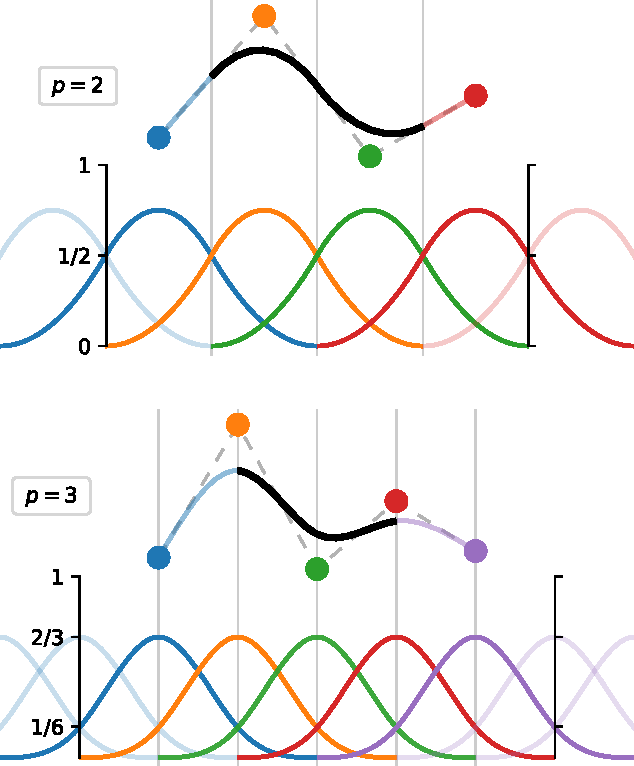
\includegraphics[width=.85\linewidth]{power/basis.pdf}
  \caption[B-spline basis functions]{Examples of two open uniform B-splines and their basis functions below. Control points are spaced evenly along the x-axis such that knots (vertical lines) align with their associated segments. The top spline is quadratic (degree $p=2$), while the bottom is cubic ($p=3$). In both, the left- and rightmost basis functions go to zero at the middle knot, and so another curve that shares the middle $p$ control points is guaranteed to overlap exactly at that knot. Note that the sum of basis functions must always add up to one, so to attach a curve to its endpoints, the final control point is repeated $p$ times. The curves there are also slightly transparent, to match the corresponding repeated basis functions.}
  \label{fig:basis}
\end{figure}

In practice this second method makes the rendered curve hug its path through the routing graph closer than the first. In the case of cubic splines ($p=3$), this means that edges come sufficiently close to look bundled, even though the above proof demonstrates that the degree must be $p=2$ for curves to fully overlap (unless routing nodes are split twice to guarantee three shared control points).
This appears to be the choice of the original authors \cite{Bach2017} in their provided source code.
The benefit of cubic splines is that they are $C^2$ continuous, i.e.\  have no sudden jumps in curvature, and having this extra smoothness is more aesthetically pleasing. Regardless, for all figures here except for the bottom of Figure~\ref{fig:basis} quadratic splines are used, along with the first method of joining to end points.

Note that drawing a spline for every edge is not the only way to render the graph, and also introduces a great deal of redundancy due to the large amount of overlapping portions. If a purely confluent drawing is desired, then it is not necessary to redraw overlapping segments.
Allowing bundles to be relaxed \cite[Fig.~18]{Bach2017} is, however, a useful option that rendering each link does provide.

\subsection{Directed graphs}
\label{sec:power_directed}
The definition for a directed confluent drawing is almost the same as the undirected case, except with the caveat that any path can only `flow' in one direction. This is analogous to preventing trains on tracks from crashing into each other. 
Formally, for a directed confluent drawing $B$, this is extra condition \cite{Dickerson2005} is:
\begin{mdframed}[backgroundcolor=WhiteSmoke]
\begin{itemize}[leftmargin=*]
  \item Locally monotone curves in B may share some overlapping portions, but the edges sharing the same portion of a track must all have the same direction along that portion.
\end{itemize}
\end{mdframed}
This means that directed graphs lead to a slightly different power-to-routing graph conversion, where the description in \cite{Bach2017} says \emph{``The only difference is that we create --- as necessary --- two junctions for each group, one for incoming and one for outgoing edges."}
Here this short description will be elaborated upon, as simply adding another routing node when its corresponding group has both incoming and outgoing edges is not enough to guarantee that all portions will only flow in one direction.
This is because any power edges at a power group are propagated down the hierarchy, so that even if flows are correctly directed into separate junctions at one group, they may still clash further down the tree.
Therefore, all descendants of any such group must also have two routing nodes: one for outgoing edges (flowing up the hierarchy) and one for incoming edges (flowing down the hierarchy).

The description of the improved power graph construction algorithm from Section~\ref{sec:power_graph} is also easily applied to directed graphs, by splitting neighbour sets into incoming and outgoing edges. This is how the original algorithm is described by Dwyer et al. \cite{Dwyer2014}.
In other words, the formulations for the heuristics in Equation~\eqref{eq:kappa_full} instead become
\begin{align}
  &\kappa_\cap(m,n) = |N^+(m)\cap N^+(n)| + |N^-(m)\cap N^-(n)|,\\
  &\kappa_{\Triangle}(m,n) = |N^+(m)\,\Triangle\,N^+(n)| + |N^-(m)\,\Triangle\,N^-(n)|
\end{align}
where $N^+$ is a set of outgoing edges, and $N^-$ a set of incoming edges.

\subsection{Planarity}
\label{sec:power_planarity}
Here the third condition in the confluent definition (Section~\ref{sec:confluent_definition}) will be discussed, which requires planarity. Unfortunately, the method of Bach et al.\ \cite{Bach2017} does not offer any guarantee of planarity due to the use of a force-directed method to lay out the graph.
While the authors do recognize this, and make the distinction that their drawings are `non-planar confluent', the loss of this condition means that almost any drawing, with or without curved edges, satisfies a now-trivial definition.
There also exist graphs that have been proven to not admit any confluent drawing \cite{Dickerson2005}, and so it is impossible for any algorithm to produce confluent drawings for general graphs.
However, the planarity condition can be relaxed in the context of finding a drawing that reduces the number of crossings, for example in layered confluent drawings \cite{Eppstein2007}. Bach et al.\ \cite{Bach2017} do not explicitly address this question, but in practice the approach can greatly reduce the number of crossings, making it a practical method to enhance readability.

Furthermore, it is easy to see that a planar ARG can always lead to a planar drawing, as long as one is careful to avoid crossings at routing nodes (which is always possible because every routing node is simply a single junction). If it is assumed that there are no redundant routing edges without adjacencies routed through them, this means that the complete confluent definition can be satisfied if and only if the ARG is also planar.
This naturally implies a new subset of confluent drawings, much like the $\Delta$-confluent \cite{Eppstein2005} or strict confluent \cite{Eppstein2013} subclasses, which can be found only through a planar power-to-routing graph conversion. Such drawings will be named \emph{power-confluent}.
This new classification will now be proven to be a subclass of strict confluent drawing. 

\subsubsection{Stricter than strict}
The definition of strict confluent drawing has only the additional restriction that there can be at most one smooth path between vertices, and there cannot be any paths from a vertex to itself \cite{Eppstein2013}. 
% For the power-confluent case, because each routing node can only have one parent, and each path must go up the tree through this parent, there can only ever be one path that can be taken between two vertices. Every power-confluent drawing is therefore also strict confluent.
For the power-confluent case, because the mapping of edges to power edges is surjective \cite{Royer2008}, each edge can only correspond to a single path through the power graph hierarchy, and therefore also through the routing graph behind the confluent drawing. Every power-confluent drawing without self-loops is therefore also strict confluent.

The reverse is not true, because another condition of power graphs is that groups must be disjoint \cite{Royer2008}, i.e.\ their boundaries may not overlap.
There exist confluent drawings that cannot result from power graphs unless this condition is broken, for example the tetrahedron-like structure in Figure~\ref{fig:strict}.
In this structure there are six junctions, and so at least six power groups are required in the corresponding power graph; however, there is a maximum of four that will not overlap, as there can only be one for each `corner' of the `tetrahedron'. This is due to the middle vertex of each `corner' sharing junctions with all three surrounding it, which means that grouping any of the three valid pairings will block out the other two.
Note that the graph itself is not necessarily impossible to draw in a power-confluent manner, but that this particular drawing could never result from the algorithm presented in this paper.
Power-confluent is therefore a strictly stronger condition than strict confluent.

\begin{figure}
  \centering
  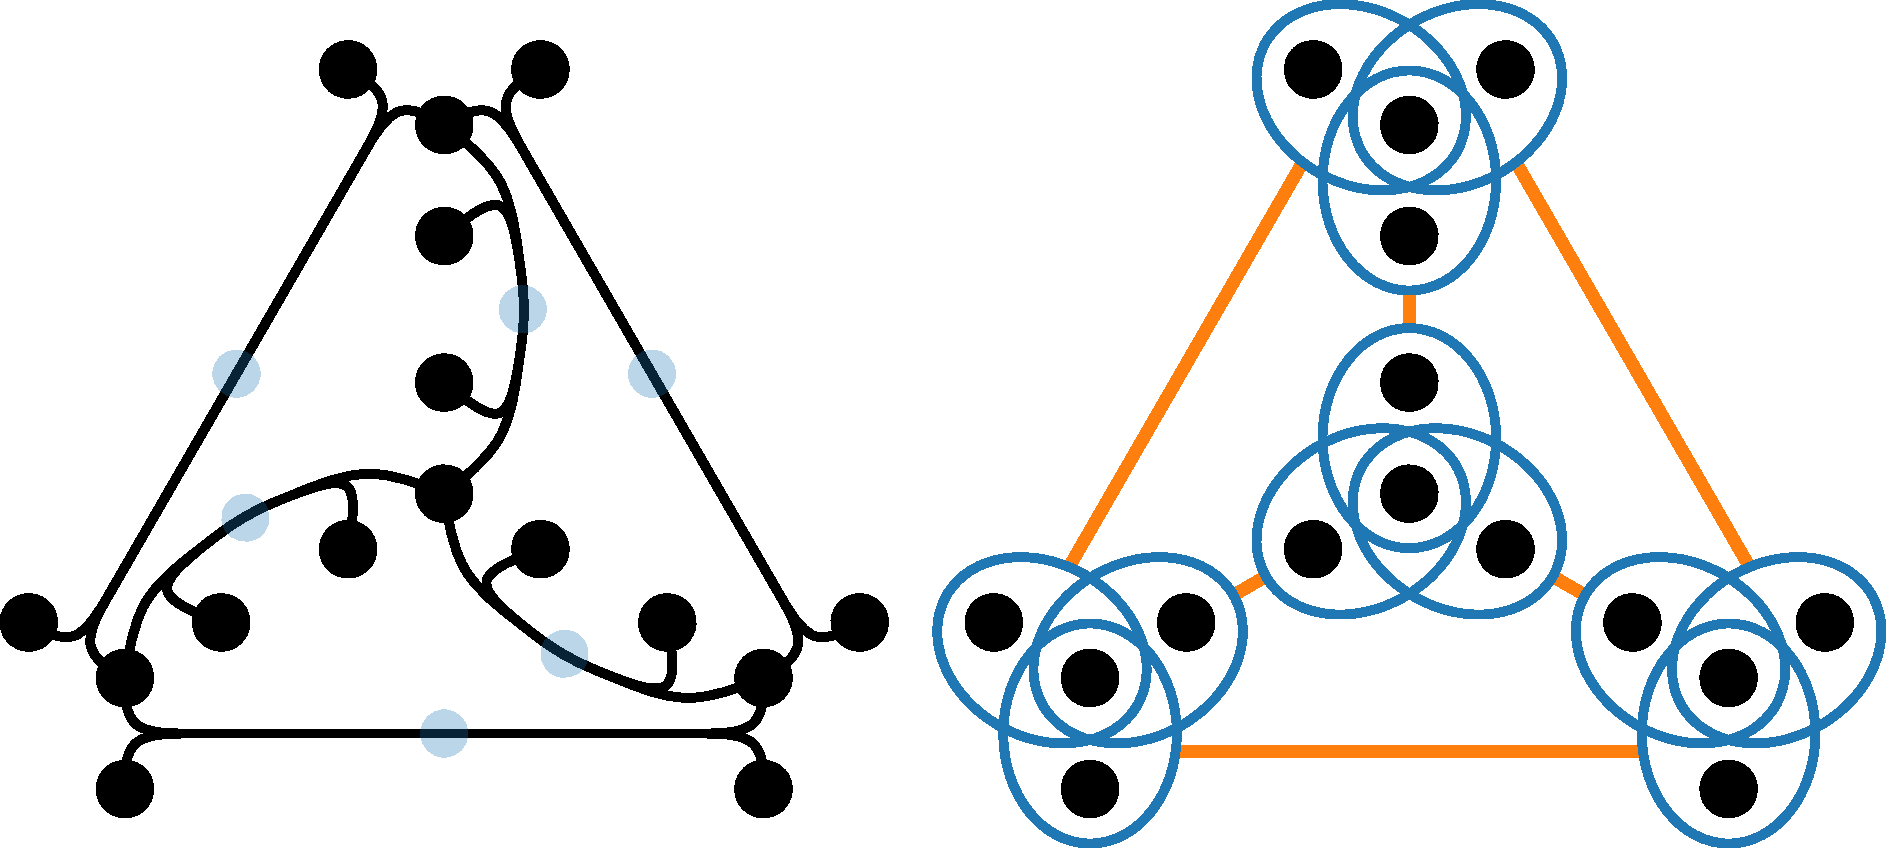
\includegraphics[width=\linewidth]{power/stricter.pdf}
  \caption[A strict confluent drawing that is not power-confluent]{An example of a strict confluent drawing that cannot be reverse-engineered into a valid power graph, unless power group boundaries are allowed to overlap. On the left is the confluent drawing (with junctions marked by transparent blue circles), and on the right is a power graph that shows all possible groupings to match these junctions. The proof is further explained in Section~\ref{sec:power_planarity}.}
  \label{fig:strict}
\end{figure}

\subsection{Discussion}
\label{sec:power_discussion}
The work presented here has developed the ideas presented by Bach et al.\ \cite{Bach2017} by both improving the power graph decomposition step (Section~\ref{sec:power_graph}) and fixing some practical issues with the conversion to a confluent drawing (Section~\ref{sec:confluent_definition}. Source code for all the algorithms discussed can be found at \url{www.github.com/jxz12/pconfluent}.

Further directions could involve developing methods to find power-confluent drawings, by guiding the search algorithm towards solutions that produce planar routing graphs.
Methods such as Monte Carlo or A* search may prove useful for either finding such drawings, or just improving the greedy search presented here.
% A different optimization heuristic may also lead to less cluttered drawings, as a well compressed power graph may not lead to a good confluent drawing. Perhaps measure the number of junctions in the resulting graph or something
% As mentioned above, proving or disproving an equivalence to strict confluent drawing is also left open. If power-confluent is a stronger condition than strict confluent, then

On the theoretical side, it may be the case that relaxing the non-overlapping group boundary condition, as explored by Ahnert \cite{Ahnert2014}, could result in an equivalent classification to strict confluent drawing.
The potential proof or refutation of this equivalence is left as an open question, along with determining the exact relationship between power decomposition and confluent drawing in general.

\begin{figure}
  \centering
  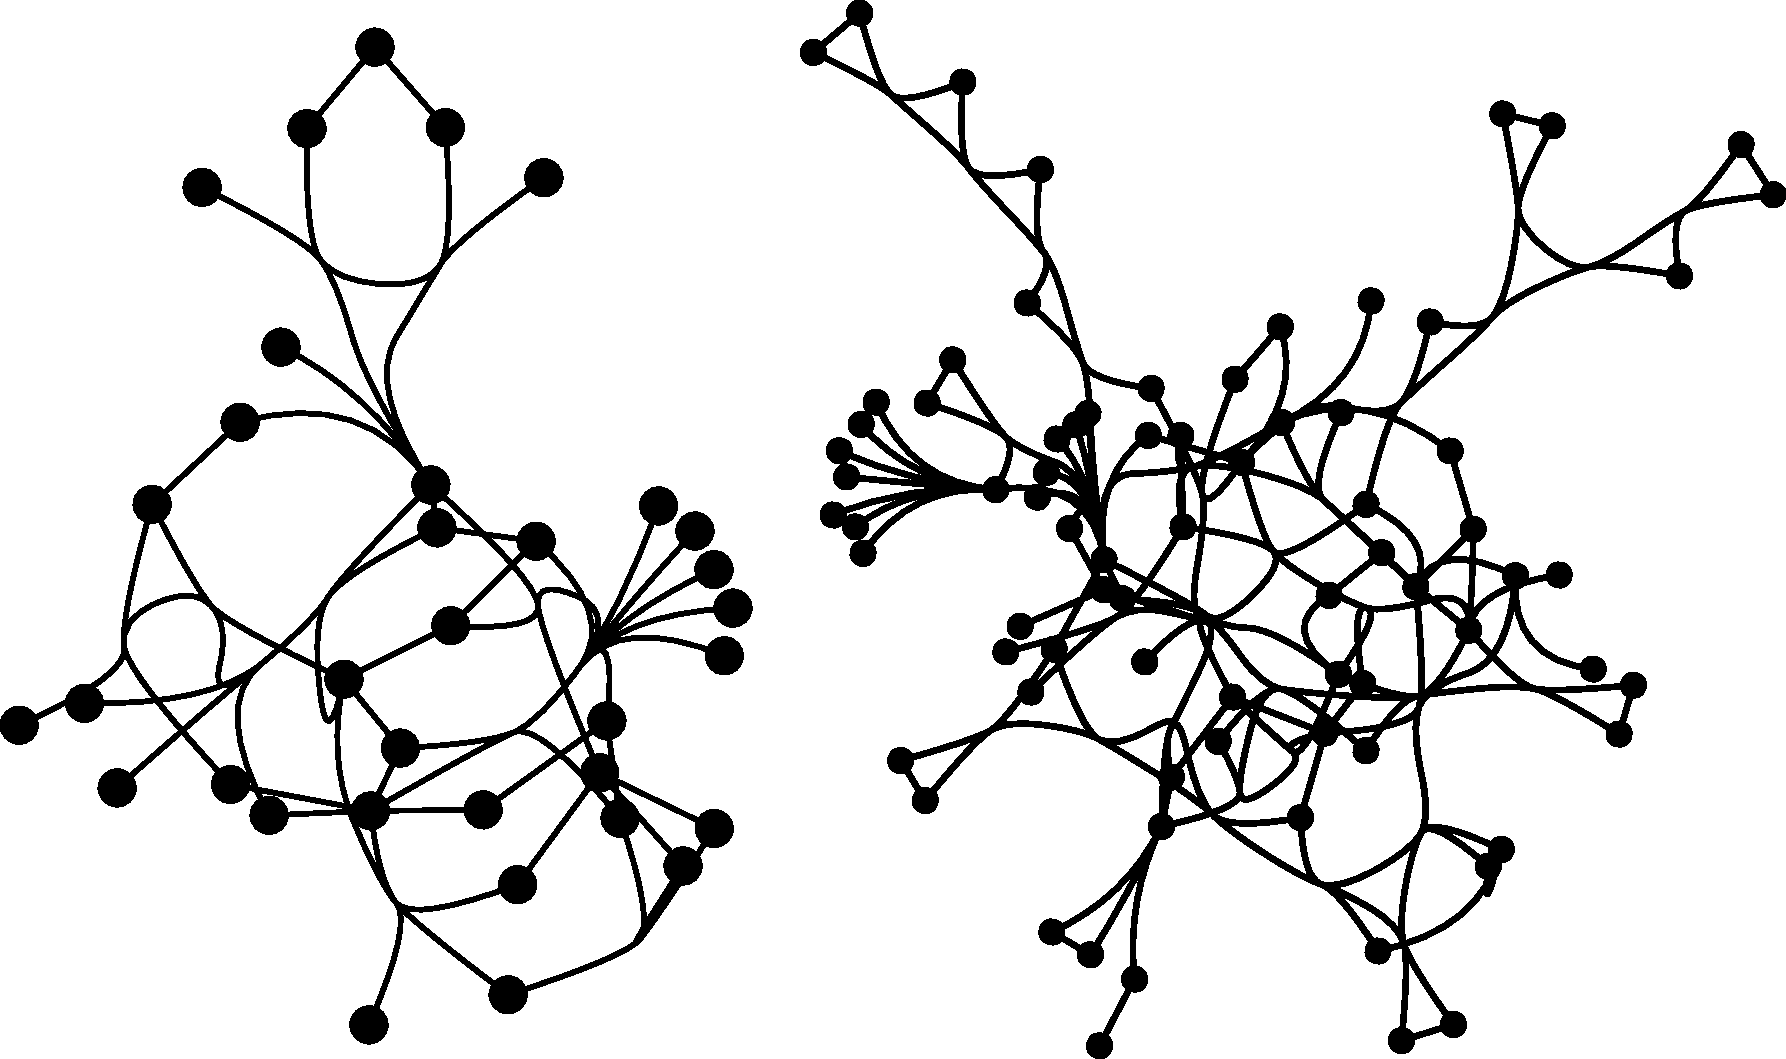
\includegraphics[width=\linewidth]{power/power_karate_lesmis.pdf}
  \caption[Examples of networks drawn with the power-confluent algorithm]{Two examples of graphs drawn with Algorithms~\ref{alg:pgd} then~\ref{alg:pcd}, in Figures~\ref{fig:pseudo_pgd} and~\ref{fig:pseudo_pcd} respectively. On the left is \texttt{karate}, previously shown in Figure~\ref{fig:untangled_hairballs}, top. On the right is \texttt{lesmis}, previously shown in Figure~\ref{fig:lesmis}.}
  \label{fig:power_karate_lesmis}
\end{figure}

To finish on a practical note, a more tailored layout algorithm than standard force-directed methods will be necessary for the algorithm to become a truly practical tool, as layouts can often become tangled and unreadable. See Figure~\ref{fig:power_karate_lesmis} for two examples of this on graphs previously studied in this chapter.
The layout function (Figure~\ref{fig:pseudo_pcd}, line~\ref{code:pcd:sgd}) is currently only given the routing graph as input, but may benefit from extra information, such as which edges are power edges and which are hierarchical. An effective radial layout that can avoid crossings, like the one shown in Figure~\ref{fig:radial} but automatic, may also offer a superior solution.
